\documentclass[twoside]{article}

% Packages required by doxygen
\usepackage{calc}
\usepackage{doxygen}
\usepackage{graphicx}
\usepackage[utf8]{inputenc}
\usepackage{makeidx}
\usepackage{multicol}
\usepackage{multirow}
\usepackage{textcomp}
\usepackage[table]{xcolor}

% NLS support packages
\usepackage[spanish]{babel}
% Font selection
\usepackage[T1]{fontenc}
\usepackage{mathptmx}
\usepackage[scaled=.90]{helvet}
\usepackage{courier}
\usepackage{amssymb}
\usepackage{sectsty}
\renewcommand{\familydefault}{\sfdefault}
\allsectionsfont{%
  \fontseries{bc}\selectfont%
  \color{darkgray}%
}
\renewcommand{\DoxyLabelFont}{%
  \fontseries{bc}\selectfont%
  \color{darkgray}%
}

% Page & text layout
\usepackage{geometry}
\geometry{%
  a4paper,%
  top=2.5cm,%
  bottom=2.5cm,%
  left=2.5cm,%
  right=2.5cm%
}
\tolerance=750
\hfuzz=15pt
\hbadness=750
\setlength{\emergencystretch}{15pt}
\setlength{\parindent}{0cm}
\setlength{\parskip}{0.2cm}
\makeatletter
\renewcommand{\paragraph}{%
  \@startsection{paragraph}{4}{0ex}{-1.0ex}{1.0ex}{%
    \normalfont\normalsize\bfseries\SS@parafont%
  }%
}
\renewcommand{\subparagraph}{%
  \@startsection{subparagraph}{5}{0ex}{-1.0ex}{1.0ex}{%
    \normalfont\normalsize\bfseries\SS@subparafont%
  }%
}
\makeatother

% Headers & footers
\usepackage{fancyhdr}
\pagestyle{fancyplain}
\fancyhead[LE]{\fancyplain{}{\bfseries\thepage}}
\fancyhead[CE]{\fancyplain{}{}}
\fancyhead[RE]{\fancyplain{}{\bfseries\leftmark}}
\fancyhead[LO]{\fancyplain{}{\bfseries\rightmark}}
\fancyhead[CO]{\fancyplain{}{}}
\fancyhead[RO]{\fancyplain{}{\bfseries\thepage}}
\fancyfoot[LE]{\fancyplain{}{}}
\fancyfoot[CE]{\fancyplain{}{}}
\fancyfoot[RE]{\fancyplain{}{\bfseries\scriptsize Generado Marzo de 2014 para Clustering por Doxygen }}
\fancyfoot[LO]{\fancyplain{}{\bfseries\scriptsize Generado Marzo de 2014 para Clustering por Doxygen }}
\fancyfoot[CO]{\fancyplain{}{}}
\fancyfoot[RO]{\fancyplain{}{}}
\renewcommand{\footrulewidth}{0.4pt}
\renewcommand{\sectionmark}[1]{%
  \markright{\thesection\ #1}%
}

% Indices & bibliography
\usepackage{natbib}
\usepackage[titles]{tocloft}
\setcounter{tocdepth}{3}
\setcounter{secnumdepth}{5}
\makeindex

% Hyperlinks (required, but should be loaded last)
\usepackage{ifpdf}
\ifpdf
  \usepackage[pdftex,pagebackref=true]{hyperref}
\else
  \usepackage[ps2pdf,pagebackref=true]{hyperref}
\fi
\hypersetup{%
  colorlinks=true,%
  linkcolor=blue,%
  citecolor=blue,%
  unicode%
}

% Custom commands
\newcommand{\clearemptydoublepage}{%
  \newpage{\pagestyle{empty}\cleardoublepage}%
}


%===== C O N T E N T S =====

\begin{document}

% Titlepage & ToC
\hypersetup{pageanchor=false}
\pagenumbering{roman}
\begin{titlepage}
\vspace*{7cm}
\begin{center}%
{\Large Clustering }\\
\vspace*{1cm}
{\large Generado por Doxygen 1.8.4}\\
\vspace*{0.5cm}
{\small Marzo de 2014}\\
\end{center}
\end{titlepage}
\tableofcontents
\pagenumbering{arabic}
\hypersetup{pageanchor=true}

%--- Begin generated contents ---
\section{Indice de namespaces}
\subsection{Lista de 'namespaces'}
Lista de los 'namespaces', con una breve descripción\-:\begin{DoxyCompactList}
\item\contentsline{section}{\hyperlink{namespace_ui}{Ui} }{\pageref{namespace_ui}}{}
\end{DoxyCompactList}

\section{Indice jerárquico}
\subsection{Jerarquía de la clase}
Esta lista de herencias esta ordenada aproximadamente por orden alfabético\-:\begin{DoxyCompactList}
\item \contentsline{section}{Algoritmo}{\pageref{class_algoritmo}}{}
\item \contentsline{section}{Cromosoma}{\pageref{class_cromosoma}}{}
\item \contentsline{section}{Lectora\-Archivo}{\pageref{class_lectora_archivo}}{}
\item Q\-Main\-Window\begin{DoxyCompactList}
\item \contentsline{section}{Main\-Window}{\pageref{class_main_window}}{}
\end{DoxyCompactList}
\end{DoxyCompactList}

\section{Índice de clases}
\subsection{Lista de clases}
Lista de las clases, estructuras, uniones e interfaces con una breve descripción\-:\begin{DoxyCompactList}
\item\contentsline{section}{\hyperlink{class_algoritmo}{Algoritmo} }{\pageref{class_algoritmo}}{}
\item\contentsline{section}{\hyperlink{class_cromosoma}{Cromosoma} }{\pageref{class_cromosoma}}{}
\item\contentsline{section}{\hyperlink{class_lectora_archivo}{Lectora\-Archivo} }{\pageref{class_lectora_archivo}}{}
\item\contentsline{section}{\hyperlink{class_main_window}{Main\-Window} }{\pageref{class_main_window}}{}
\end{DoxyCompactList}

\section{Indice de archivos}
\subsection{Lista de archivos}
Lista de todos los archivos con descripciones breves\-:\begin{DoxyCompactList}
\item\contentsline{section}{clustering/\hyperlink{algoritmo_8cpp}{algoritmo.\-cpp} \\*Implementaci\'{o}n de los mtodos de la clase \hyperlink{class_algoritmo}{Algoritmo} }{\pageref{algoritmo_8cpp}}{}
\item\contentsline{section}{clustering/\hyperlink{algoritmo_8h}{algoritmo.\-h} \\*Definici\'{o}n de la clase \hyperlink{class_algoritmo}{Algoritmo} }{\pageref{algoritmo_8h}}{}
\item\contentsline{section}{clustering/\hyperlink{cromosoma_8cpp}{cromosoma.\-cpp} \\*Implementaci\'{o}n de los mtodos de la clase \hyperlink{class_cromosoma}{Cromosoma} }{\pageref{cromosoma_8cpp}}{}
\item\contentsline{section}{clustering/\hyperlink{cromosoma_8h}{cromosoma.\-h} \\*Definici\'{o}n de la clase \hyperlink{class_cromosoma}{Cromosoma} }{\pageref{cromosoma_8h}}{}
\item\contentsline{section}{clustering/\hyperlink{lectoraarchivo_8cpp}{lectoraarchivo.\-cpp} \\*Implementaci\'{o}n de los mtodos de la clase \hyperlink{class_lectora_archivo}{Lectora\-Archivo} }{\pageref{lectoraarchivo_8cpp}}{}
\item\contentsline{section}{clustering/\hyperlink{lectoraarchivo_8h}{lectoraarchivo.\-h} \\*Definici\'{o}n de la clase \hyperlink{class_lectora_archivo}{Lectora\-Archivo} }{\pageref{lectoraarchivo_8h}}{}
\item\contentsline{section}{clustering/\hyperlink{main_8cpp}{main.\-cpp} \\*Archivo principal del proyecto }{\pageref{main_8cpp}}{}
\item\contentsline{section}{clustering/\hyperlink{mainwindow_8cpp}{mainwindow.\-cpp} \\*Implementaci\'{o}n de los mtodos de la clase \hyperlink{class_main_window}{Main\-Window} }{\pageref{mainwindow_8cpp}}{}
\item\contentsline{section}{clustering/\hyperlink{mainwindow_8h}{mainwindow.\-h} \\*Definici\'{o}n de la clase \hyperlink{class_main_window}{Main\-Window} }{\pageref{mainwindow_8h}}{}
\end{DoxyCompactList}

\section{Documentación de namespaces}
\hypertarget{namespace_ui}{\subsection{Referencia del Namespace Ui}
\label{namespace_ui}\index{Ui@{Ui}}
}

\section{Documentación de las clases}
\hypertarget{class_algoritmo}{\subsection{Referencia de la Clase Algoritmo}
\label{class_algoritmo}\index{Algoritmo@{Algoritmo}}
}


{\ttfamily \#include $<$algoritmo.\-h$>$}

\subsubsection*{Métodos públicos}
\begin{DoxyCompactItemize}
\item 
\hyperlink{class_algoritmo_a19b6e2a6788c748669bf22507198c00d}{Algoritmo} ()
\begin{DoxyCompactList}\small\item\em \hyperlink{class_algoritmo_a19b6e2a6788c748669bf22507198c00d}{Algoritmo\-::\-Algoritmo()} Contructor por defecto. Inicializa un objeto \hyperlink{class_algoritmo}{Algoritmo}. \end{DoxyCompactList}\item 
\hyperlink{class_algoritmo_ae43b195db4527bb14eb4be2343908730}{Algoritmo} (igraph\-\_\-t \&\hyperlink{class_algoritmo_a5bf75458f302256836f8c021c696b6d6}{grafo}, int \hyperlink{class_algoritmo_a8b600a2b305e168f34896450a86330de}{nodos}, int \hyperlink{class_algoritmo_aebd547b83ffc0fc84727b4d32816e6a3}{aristas}, int \hyperlink{class_algoritmo_a5b2603327a6c450a76a6852ac26fe7a2}{individuos}, int \hyperlink{class_algoritmo_a76362b4a8f794e6206dcbeec3fe7a628}{generaciones}, double \hyperlink{class_algoritmo_a8423d3ea20137a281055f4b04f1d5492}{porcentaje\-Mating\-Pool}, bool \hyperlink{class_algoritmo_a128d4c2bd8d16eb3cb94f29f75ce33de}{mutar\-Dos\-Bits})
\begin{DoxyCompactList}\small\item\em \hyperlink{class_algoritmo_a19b6e2a6788c748669bf22507198c00d}{Algoritmo\-::\-Algoritmo} Constructor. Inicializa un objeto \hyperlink{class_algoritmo}{Algoritmo}. \end{DoxyCompactList}\item 
\hyperlink{class_algoritmo_a39b97924ace4107969fb6702b8ec11b7}{$\sim$\-Algoritmo} ()
\item 
void \hyperlink{class_algoritmo_a2af7a7e2b849e950a40edb29dbe48ee1}{algoritmo} ()
\begin{DoxyCompactList}\small\item\em \hyperlink{class_algoritmo_a2af7a7e2b849e950a40edb29dbe48ee1}{Algoritmo\-::algoritmo} Se realiza primero el {\itshape clustering} haciendo uso del algoritmo de Newman. Paso siguiente se inicializa la poblaci\'{o}n de cromosomas garantizando que tengan solapamiento entre {\itshape clusters}. Luego de tener la poblaci\'{o}n inicial, se realiza la selecci\'{o}n de un porcentaje de cromosomas, usando la modularidad como funci\'{o}n de aptitud. Una vez se carga el {\itshape mating pool} con los cromosomas seleccionados se realiza la reproducci\'{o}n, usando como operador la mutaci\'{o}n.\par
 Finalmente se selecciona como soluci\'{o}n el cromosoma que obtenga la mayor modularidad. \end{DoxyCompactList}\item 
double \hyperlink{class_algoritmo_ab547948993b374fb0721c1f7ec46ded8}{get\-Modularidad} ()
\begin{DoxyCompactList}\small\item\em \hyperlink{class_algoritmo_ab547948993b374fb0721c1f7ec46ded8}{Algoritmo\-::get\-Modularidad} Retorna la modularidad final obtenida con el mejor cromosoma encontrado. \end{DoxyCompactList}\item 
vector$<$ unordered\-\_\-set$<$ int $>$ $>$ \hyperlink{class_algoritmo_a02ba46efa94c279b129c92365a6a369c}{get\-Configuracion\-Final} ()
\begin{DoxyCompactList}\small\item\em \hyperlink{class_algoritmo_a02ba46efa94c279b129c92365a6a369c}{Algoritmo\-::get\-Configuracion\-Final} Retorna la configuraci\'{o}n final del mejor cromosoma encontrado. \end{DoxyCompactList}\item 
int \hyperlink{class_algoritmo_a58bbe61d845ba28704b4b44e74f89b6c}{get\-Cant\-Cambios} ()
\begin{DoxyCompactList}\small\item\em \hyperlink{class_algoritmo_a58bbe61d845ba28704b4b44e74f89b6c}{Algoritmo\-::get\-Cant\-Cambios} Retorna cuantos cambios se hicieron a la referencia del mejor cromosoma al final del algoritmo (Para elegir la soluci\'{o}n). \end{DoxyCompactList}\end{DoxyCompactItemize}
\subsubsection*{Métodos privados}
\begin{DoxyCompactItemize}
\item 
void \hyperlink{class_algoritmo_a31e6f36a2b008ec1b777f2bea78cdcb9}{inicializar\-Poblacion} ()
\begin{DoxyCompactList}\small\item\em \hyperlink{class_algoritmo_a31e6f36a2b008ec1b777f2bea78cdcb9}{Algoritmo\-::inicializar\-Poblacion} Se crean los individuos iniciales de cromosomas, se usa la configuraci\'{o}n de {\itshape clustering} retornada por Newman, y se garantiza que todos los cromosomas iniciales tengan solapamiento en un nodo. \end{DoxyCompactList}\item 
void \hyperlink{class_algoritmo_a0ea4f57c37e4a6fc36a189b1fb72f2f5}{seleccionar} ()
\begin{DoxyCompactList}\small\item\em \hyperlink{class_algoritmo_a0ea4f57c37e4a6fc36a189b1fb72f2f5}{Algoritmo\-::seleccionar} La selecci\'{o}n se realiza con la t\'{e}cnica torneo, se seleccionan dos cromosomas al azar, de cada uno se obtiene la modularidad, se elige el cromosoma con mayor modularidad. Si la modularidad llegara a ser igual en ambos cromosomas, se elige el cromosoma que tenga mayor porcentaje de {\itshape clusters} respecto a la cantidad de {\itshape clusters} encontrada al inicio con el algoritmo de Newman. \par
 \end{DoxyCompactList}\item 
void \hyperlink{class_algoritmo_ac8d6cb1e51861008c6d50ab9e8b3666a}{reproducir} ()
\begin{DoxyCompactList}\small\item\em \hyperlink{class_algoritmo_ac8d6cb1e51861008c6d50ab9e8b3666a}{Algoritmo\-::reproducir} Para la reproducci\'{o}n, se usa la mutaci\'{o}n sobre un cromosoma, esta puede darse de dos formas, seg\'{u}n el se halla definido. Una es mutar un solo {\itshape bit} de la matriz X, y la otra mutar dos {\itshape bits} de la matriz X. Si el cromosoma es el indicado por el indice del mejor cromosoma en el mating pool, este no se muta y se pasa directo a la siguiente generaci\'{o}n. \end{DoxyCompactList}\item 
void \hyperlink{class_algoritmo_a718fe5e18f1b887a7c10604935664402}{clustering\-Newman} ()
\begin{DoxyCompactList}\small\item\em \hyperlink{class_algoritmo_a718fe5e18f1b887a7c10604935664402}{Algoritmo\-::clustering\-Newman} Realiza el primer {\itshape clustering} haciendo uso del algoritmo propuesto por Newman en {\bfseries  Finding community structure in very large networks} puede ver detalles en \href{http://igraph.sourceforge.net/doc/html/ch22s06.html}{\tt http\-://igraph.\-sourceforge.\-net/doc/html/ch22s06.\-html} y \href{http://www.arxiv.org/abs/cond-mat/0408187}{\tt http\-://www.\-arxiv.\-org/abs/cond-\/mat/0408187 }. \end{DoxyCompactList}\item 
void \hyperlink{class_algoritmo_a587697ecb58bbd4f7a5bfe7188f681cb}{inicializar\-Matriz\-X} ()
\begin{DoxyCompactList}\small\item\em \hyperlink{class_algoritmo_a587697ecb58bbd4f7a5bfe7188f681cb}{Algoritmo\-::inicializar\-Matriz\-X} Inicializa la matriz de membresia (binaria), tal y como el algoritmo de Newma configur\'{o} los {\itshape clusters}. La matriz tiene la forma descrita en el trabajo \href{http://dl.acm.org/citation.cfm?id=1339693}{\tt A Extraction Method of Overlapping Cluster Based on Network Structure Analysis} Las filas corresponden a los {\itshape clusters} y las columnas a los nodos. \end{DoxyCompactList}\item 
void \hyperlink{class_algoritmo_a3fd78d6f0173d1f25ea0fc6437fa151d}{inicializar\-Configuracion\-Inicial} ()
\begin{DoxyCompactList}\small\item\em \hyperlink{class_algoritmo_a3fd78d6f0173d1f25ea0fc6437fa151d}{Algoritmo\-::inicializar\-Configuracion\-Inicial} Inicializa la configuraci\'{o}n incial de {\itshape clustering} en el formato de lista de adyacencia. \end{DoxyCompactList}\item 
void \hyperlink{class_algoritmo_a4be398fd15aaf32dc7b279ebc5ea90d7}{construir\-Lista\-Adyacencia} ()
\begin{DoxyCompactList}\small\item\em \hyperlink{class_algoritmo_a4be398fd15aaf32dc7b279ebc5ea90d7}{Algoritmo\-::construir\-Lista\-Adyacencia} Crea la lista de adyacencia del grafo, la cual corresponde a una estructura de dato mucho m\'{a}s eficiente que la matriz de adyacencia. Se usa como estructura de dato vector$<$unordered\-\_\-set$<$int$>$$>$. \end{DoxyCompactList}\end{DoxyCompactItemize}
\subsubsection*{Atributos privados}
\begin{DoxyCompactItemize}
\item 
int \hyperlink{class_algoritmo_a8b600a2b305e168f34896450a86330de}{nodos}
\item 
int \hyperlink{class_algoritmo_aebd547b83ffc0fc84727b4d32816e6a3}{aristas}
\item 
int \hyperlink{class_algoritmo_a5b2603327a6c450a76a6852ac26fe7a2}{individuos}
\item 
int \hyperlink{class_algoritmo_a76362b4a8f794e6206dcbeec3fe7a628}{generaciones}
\item 
\hyperlink{class_cromosoma}{Cromosoma} $\ast$$\ast$ \hyperlink{class_algoritmo_a5f6b839180abb11469b6e33cf2dd2871}{poblacion}
\item 
\hyperlink{class_cromosoma}{Cromosoma} $\ast$$\ast$ \hyperlink{class_algoritmo_a9c6c102ca50a3d69052d3c06ef19725c}{mating\-Pool}
\item 
int \hyperlink{class_algoritmo_aeda95cdb4165c41656c1a3e2e157eb51}{mejor\-Indice\-Poblacion}
\item 
double \hyperlink{class_algoritmo_a282ec70d907d6923b59c91e425ad493f}{mejor\-Modularidad}
\item 
\hyperlink{class_cromosoma}{Cromosoma} $\ast$ \hyperlink{class_algoritmo_a2bb44f3dd4096ece8959ed32b05b5147}{mejor\-Cromosoma}
\item 
int \hyperlink{class_algoritmo_a0c34d9a4f7a55fc4afa538dd477ac633}{tam\-Mating\-Pool}
\item 
double \hyperlink{class_algoritmo_a8423d3ea20137a281055f4b04f1d5492}{porcentaje\-Mating\-Pool}
\item 
bool \hyperlink{class_algoritmo_a128d4c2bd8d16eb3cb94f29f75ce33de}{mutar\-Dos\-Bits}
\item 
igraph\-\_\-t \hyperlink{class_algoritmo_a5bf75458f302256836f8c021c696b6d6}{grafo}
\item 
double \hyperlink{class_algoritmo_a2aff6cb6814150fe6abdf5a3458765f8}{modularidad\-Inicial}
\item 
double \hyperlink{class_algoritmo_ad31bad8b81588053130542bc3ffb3d06}{modularidad\-Final}
\item 
int \hyperlink{class_algoritmo_a740325de9f0e126452afbf5bce34bbc7}{cant\-Clusters\-Inicial}
\item 
int \hyperlink{class_algoritmo_a4b3baaedefed9ee655a1d1819b78a5df}{cant\-Cambios}
\item 
igraph\-\_\-vector\-\_\-t \hyperlink{class_algoritmo_aa4b30738a2e2676d8375ad8a465067a7}{tamanio\-Clusters\-Inicial}
\item 
igraph\-\_\-vector\-\_\-t \hyperlink{class_algoritmo_ada55baff2fa6f00d257d2af78ba10b18}{membresia\-Inicial}
\item 
vector$<$ vector$<$ bool $>$ $>$ \hyperlink{class_algoritmo_a2d2c192209608ebd713ccdd2460a1778}{matriz\-X\-Inicial}
\item 
vector$<$ unordered\-\_\-set$<$ int $>$ $>$ \hyperlink{class_algoritmo_a12d991b910cdf5383a53b1b7c12bad40}{configuracion\-Inicial}
\item 
vector$<$ unordered\-\_\-set$<$ int $>$ $>$ \hyperlink{class_algoritmo_a93ba06ec3089ad3b17037b2432136477}{lista\-Adyacencia}
\item 
vector$<$ unordered\-\_\-set$<$ int $>$ $>$ \hyperlink{class_algoritmo_ac1129d6d9bc8bc6e731b0ad24ecb799a}{configuracion\-Final}
\end{DoxyCompactItemize}


\subsubsection{Descripción detallada}


Definición en la línea 19 del archivo algoritmo.\-h.



\subsubsection{Documentación del constructor y destructor}
\hypertarget{class_algoritmo_a19b6e2a6788c748669bf22507198c00d}{\index{Algoritmo@{Algoritmo}!Algoritmo@{Algoritmo}}
\index{Algoritmo@{Algoritmo}!Algoritmo@{Algoritmo}}
\paragraph[{Algoritmo}]{\setlength{\rightskip}{0pt plus 5cm}Algoritmo\-::\-Algoritmo (
\begin{DoxyParamCaption}
{}
\end{DoxyParamCaption}
)}}\label{class_algoritmo_a19b6e2a6788c748669bf22507198c00d}


\hyperlink{class_algoritmo_a19b6e2a6788c748669bf22507198c00d}{Algoritmo\-::\-Algoritmo()} Contructor por defecto. Inicializa un objeto \hyperlink{class_algoritmo}{Algoritmo}. 



Definición en la línea 20 del archivo algoritmo.\-cpp.

\hypertarget{class_algoritmo_ae43b195db4527bb14eb4be2343908730}{\index{Algoritmo@{Algoritmo}!Algoritmo@{Algoritmo}}
\index{Algoritmo@{Algoritmo}!Algoritmo@{Algoritmo}}
\paragraph[{Algoritmo}]{\setlength{\rightskip}{0pt plus 5cm}Algoritmo\-::\-Algoritmo (
\begin{DoxyParamCaption}
\item[{igraph\-\_\-t \&}]{grafo, }
\item[{int}]{nodos, }
\item[{int}]{aristas, }
\item[{int}]{individuos, }
\item[{int}]{generaciones, }
\item[{double}]{porcentaje\-Mating\-Pool, }
\item[{bool}]{mutar\-Dos\-Bits}
\end{DoxyParamCaption}
)}}\label{class_algoritmo_ae43b195db4527bb14eb4be2343908730}


\hyperlink{class_algoritmo_a19b6e2a6788c748669bf22507198c00d}{Algoritmo\-::\-Algoritmo} Constructor. Inicializa un objeto \hyperlink{class_algoritmo}{Algoritmo}. 


\begin{DoxyParams}{Parámetros}
{\em grafo} & igraph\-\_\-t\& grafo al cual se le realizar\'{a} el agrupamiento. \\
\hline
{\em nodos} & int con el n\'{u}mero total de nodos del grafo. \\
\hline
{\em aristas} & int con el n\'{u}mero total de aristas del grafo. \\
\hline
{\em individuos} & int cantidad de individuos para la poblaci\'{o}n inicial. \\
\hline
{\em generaciones} & int n\'{u}mero de generaciones para iterar el algoritmo. \\
\hline
{\em porcentaje\-Mating\-Pool} & double con el porcentaje de la poblaci\'{o}n inicial que se llevar\'{a} al {\itshape mating pool} \\
\hline
{\em mutar\-Dos\-Bits} & bool activa mutar sobre dos bits de la matriz de membresia, sino se muta sobre un s\'{o}lo bit. \\
\hline
\end{DoxyParams}


Definición en la línea 36 del archivo algoritmo.\-cpp.

\hypertarget{class_algoritmo_a39b97924ace4107969fb6702b8ec11b7}{\index{Algoritmo@{Algoritmo}!$\sim$\-Algoritmo@{$\sim$\-Algoritmo}}
\index{$\sim$\-Algoritmo@{$\sim$\-Algoritmo}!Algoritmo@{Algoritmo}}
\paragraph[{$\sim$\-Algoritmo}]{\setlength{\rightskip}{0pt plus 5cm}Algoritmo\-::$\sim$\-Algoritmo (
\begin{DoxyParamCaption}
{}
\end{DoxyParamCaption}
)}}\label{class_algoritmo_a39b97924ace4107969fb6702b8ec11b7}


Definición en la línea 64 del archivo algoritmo.\-cpp.



\subsubsection{Documentación de las funciones miembro}
\hypertarget{class_algoritmo_a2af7a7e2b849e950a40edb29dbe48ee1}{\index{Algoritmo@{Algoritmo}!algoritmo@{algoritmo}}
\index{algoritmo@{algoritmo}!Algoritmo@{Algoritmo}}
\paragraph[{algoritmo}]{\setlength{\rightskip}{0pt plus 5cm}void Algoritmo\-::algoritmo (
\begin{DoxyParamCaption}
{}
\end{DoxyParamCaption}
)}}\label{class_algoritmo_a2af7a7e2b849e950a40edb29dbe48ee1}


\hyperlink{class_algoritmo_a2af7a7e2b849e950a40edb29dbe48ee1}{Algoritmo\-::algoritmo} Se realiza primero el {\itshape clustering} haciendo uso del algoritmo de Newman. Paso siguiente se inicializa la poblaci\'{o}n de cromosomas garantizando que tengan solapamiento entre {\itshape clusters}. Luego de tener la poblaci\'{o}n inicial, se realiza la selecci\'{o}n de un porcentaje de cromosomas, usando la modularidad como funci\'{o}n de aptitud. Una vez se carga el {\itshape mating pool} con los cromosomas seleccionados se realiza la reproducci\'{o}n, usando como operador la mutaci\'{o}n.\par
 Finalmente se selecciona como soluci\'{o}n el cromosoma que obtenga la mayor modularidad. 



Definición en la línea 102 del archivo algoritmo.\-cpp.

\hypertarget{class_algoritmo_a718fe5e18f1b887a7c10604935664402}{\index{Algoritmo@{Algoritmo}!clustering\-Newman@{clustering\-Newman}}
\index{clustering\-Newman@{clustering\-Newman}!Algoritmo@{Algoritmo}}
\paragraph[{clustering\-Newman}]{\setlength{\rightskip}{0pt plus 5cm}void Algoritmo\-::clustering\-Newman (
\begin{DoxyParamCaption}
{}
\end{DoxyParamCaption}
)\hspace{0.3cm}{\ttfamily [private]}}}\label{class_algoritmo_a718fe5e18f1b887a7c10604935664402}


\hyperlink{class_algoritmo_a718fe5e18f1b887a7c10604935664402}{Algoritmo\-::clustering\-Newman} Realiza el primer {\itshape clustering} haciendo uso del algoritmo propuesto por Newman en {\bfseries  Finding community structure in very large networks} puede ver detalles en \href{http://igraph.sourceforge.net/doc/html/ch22s06.html}{\tt http\-://igraph.\-sourceforge.\-net/doc/html/ch22s06.\-html} y \href{http://www.arxiv.org/abs/cond-mat/0408187}{\tt http\-://www.\-arxiv.\-org/abs/cond-\/mat/0408187 }. 



Definición en la línea 165 del archivo algoritmo.\-cpp.

\hypertarget{class_algoritmo_a4be398fd15aaf32dc7b279ebc5ea90d7}{\index{Algoritmo@{Algoritmo}!construir\-Lista\-Adyacencia@{construir\-Lista\-Adyacencia}}
\index{construir\-Lista\-Adyacencia@{construir\-Lista\-Adyacencia}!Algoritmo@{Algoritmo}}
\paragraph[{construir\-Lista\-Adyacencia}]{\setlength{\rightskip}{0pt plus 5cm}void Algoritmo\-::construir\-Lista\-Adyacencia (
\begin{DoxyParamCaption}
{}
\end{DoxyParamCaption}
)\hspace{0.3cm}{\ttfamily [private]}}}\label{class_algoritmo_a4be398fd15aaf32dc7b279ebc5ea90d7}


\hyperlink{class_algoritmo_a4be398fd15aaf32dc7b279ebc5ea90d7}{Algoritmo\-::construir\-Lista\-Adyacencia} Crea la lista de adyacencia del grafo, la cual corresponde a una estructura de dato mucho m\'{a}s eficiente que la matriz de adyacencia. Se usa como estructura de dato vector$<$unordered\-\_\-set$<$int$>$$>$. 



Definición en la línea 534 del archivo algoritmo.\-cpp.

\hypertarget{class_algoritmo_a58bbe61d845ba28704b4b44e74f89b6c}{\index{Algoritmo@{Algoritmo}!get\-Cant\-Cambios@{get\-Cant\-Cambios}}
\index{get\-Cant\-Cambios@{get\-Cant\-Cambios}!Algoritmo@{Algoritmo}}
\paragraph[{get\-Cant\-Cambios}]{\setlength{\rightskip}{0pt plus 5cm}int Algoritmo\-::get\-Cant\-Cambios (
\begin{DoxyParamCaption}
{}
\end{DoxyParamCaption}
)}}\label{class_algoritmo_a58bbe61d845ba28704b4b44e74f89b6c}


\hyperlink{class_algoritmo_a58bbe61d845ba28704b4b44e74f89b6c}{Algoritmo\-::get\-Cant\-Cambios} Retorna cuantos cambios se hicieron a la referencia del mejor cromosoma al final del algoritmo (Para elegir la soluci\'{o}n). 

\begin{DoxyReturn}{Devuelve}
int cant\-Cambios 
\end{DoxyReturn}


Definición en la línea 218 del archivo algoritmo.\-cpp.

\hypertarget{class_algoritmo_a02ba46efa94c279b129c92365a6a369c}{\index{Algoritmo@{Algoritmo}!get\-Configuracion\-Final@{get\-Configuracion\-Final}}
\index{get\-Configuracion\-Final@{get\-Configuracion\-Final}!Algoritmo@{Algoritmo}}
\paragraph[{get\-Configuracion\-Final}]{\setlength{\rightskip}{0pt plus 5cm}vector$<$ unordered\-\_\-set$<$ int $>$ $>$ Algoritmo\-::get\-Configuracion\-Final (
\begin{DoxyParamCaption}
{}
\end{DoxyParamCaption}
)}}\label{class_algoritmo_a02ba46efa94c279b129c92365a6a369c}


\hyperlink{class_algoritmo_a02ba46efa94c279b129c92365a6a369c}{Algoritmo\-::get\-Configuracion\-Final} Retorna la configuraci\'{o}n final del mejor cromosoma encontrado. 

\begin{DoxyReturn}{Devuelve}
vector$<$unordered\-\_\-set$<$int$>$ $>$ con la configuraci\'{o}n final. 
\end{DoxyReturn}


Definición en la línea 208 del archivo algoritmo.\-cpp.

\hypertarget{class_algoritmo_ab547948993b374fb0721c1f7ec46ded8}{\index{Algoritmo@{Algoritmo}!get\-Modularidad@{get\-Modularidad}}
\index{get\-Modularidad@{get\-Modularidad}!Algoritmo@{Algoritmo}}
\paragraph[{get\-Modularidad}]{\setlength{\rightskip}{0pt plus 5cm}double Algoritmo\-::get\-Modularidad (
\begin{DoxyParamCaption}
{}
\end{DoxyParamCaption}
)}}\label{class_algoritmo_ab547948993b374fb0721c1f7ec46ded8}


\hyperlink{class_algoritmo_ab547948993b374fb0721c1f7ec46ded8}{Algoritmo\-::get\-Modularidad} Retorna la modularidad final obtenida con el mejor cromosoma encontrado. 

\begin{DoxyReturn}{Devuelve}
double con la modularidad final. 
\end{DoxyReturn}


Definición en la línea 198 del archivo algoritmo.\-cpp.

\hypertarget{class_algoritmo_a3fd78d6f0173d1f25ea0fc6437fa151d}{\index{Algoritmo@{Algoritmo}!inicializar\-Configuracion\-Inicial@{inicializar\-Configuracion\-Inicial}}
\index{inicializar\-Configuracion\-Inicial@{inicializar\-Configuracion\-Inicial}!Algoritmo@{Algoritmo}}
\paragraph[{inicializar\-Configuracion\-Inicial}]{\setlength{\rightskip}{0pt plus 5cm}void Algoritmo\-::inicializar\-Configuracion\-Inicial (
\begin{DoxyParamCaption}
{}
\end{DoxyParamCaption}
)\hspace{0.3cm}{\ttfamily [private]}}}\label{class_algoritmo_a3fd78d6f0173d1f25ea0fc6437fa151d}


\hyperlink{class_algoritmo_a3fd78d6f0173d1f25ea0fc6437fa151d}{Algoritmo\-::inicializar\-Configuracion\-Inicial} Inicializa la configuraci\'{o}n incial de {\itshape clustering} en el formato de lista de adyacencia. 



Definición en la línea 500 del archivo algoritmo.\-cpp.

\hypertarget{class_algoritmo_a587697ecb58bbd4f7a5bfe7188f681cb}{\index{Algoritmo@{Algoritmo}!inicializar\-Matriz\-X@{inicializar\-Matriz\-X}}
\index{inicializar\-Matriz\-X@{inicializar\-Matriz\-X}!Algoritmo@{Algoritmo}}
\paragraph[{inicializar\-Matriz\-X}]{\setlength{\rightskip}{0pt plus 5cm}void Algoritmo\-::inicializar\-Matriz\-X (
\begin{DoxyParamCaption}
{}
\end{DoxyParamCaption}
)\hspace{0.3cm}{\ttfamily [private]}}}\label{class_algoritmo_a587697ecb58bbd4f7a5bfe7188f681cb}


\hyperlink{class_algoritmo_a587697ecb58bbd4f7a5bfe7188f681cb}{Algoritmo\-::inicializar\-Matriz\-X} Inicializa la matriz de membresia (binaria), tal y como el algoritmo de Newma configur\'{o} los {\itshape clusters}. La matriz tiene la forma descrita en el trabajo \href{http://dl.acm.org/citation.cfm?id=1339693}{\tt A Extraction Method of Overlapping Cluster Based on Network Structure Analysis} Las filas corresponden a los {\itshape clusters} y las columnas a los nodos. 



Definición en la línea 472 del archivo algoritmo.\-cpp.

\hypertarget{class_algoritmo_a31e6f36a2b008ec1b777f2bea78cdcb9}{\index{Algoritmo@{Algoritmo}!inicializar\-Poblacion@{inicializar\-Poblacion}}
\index{inicializar\-Poblacion@{inicializar\-Poblacion}!Algoritmo@{Algoritmo}}
\paragraph[{inicializar\-Poblacion}]{\setlength{\rightskip}{0pt plus 5cm}void Algoritmo\-::inicializar\-Poblacion (
\begin{DoxyParamCaption}
{}
\end{DoxyParamCaption}
)\hspace{0.3cm}{\ttfamily [private]}}}\label{class_algoritmo_a31e6f36a2b008ec1b777f2bea78cdcb9}


\hyperlink{class_algoritmo_a31e6f36a2b008ec1b777f2bea78cdcb9}{Algoritmo\-::inicializar\-Poblacion} Se crean los individuos iniciales de cromosomas, se usa la configuraci\'{o}n de {\itshape clustering} retornada por Newman, y se garantiza que todos los cromosomas iniciales tengan solapamiento en un nodo. 



Definición en la línea 229 del archivo algoritmo.\-cpp.

\hypertarget{class_algoritmo_ac8d6cb1e51861008c6d50ab9e8b3666a}{\index{Algoritmo@{Algoritmo}!reproducir@{reproducir}}
\index{reproducir@{reproducir}!Algoritmo@{Algoritmo}}
\paragraph[{reproducir}]{\setlength{\rightskip}{0pt plus 5cm}void Algoritmo\-::reproducir (
\begin{DoxyParamCaption}
{}
\end{DoxyParamCaption}
)\hspace{0.3cm}{\ttfamily [private]}}}\label{class_algoritmo_ac8d6cb1e51861008c6d50ab9e8b3666a}


\hyperlink{class_algoritmo_ac8d6cb1e51861008c6d50ab9e8b3666a}{Algoritmo\-::reproducir} Para la reproducci\'{o}n, se usa la mutaci\'{o}n sobre un cromosoma, esta puede darse de dos formas, seg\'{u}n el se halla definido. Una es mutar un solo {\itshape bit} de la matriz X, y la otra mutar dos {\itshape bits} de la matriz X. Si el cromosoma es el indicado por el indice del mejor cromosoma en el mating pool, este no se muta y se pasa directo a la siguiente generaci\'{o}n. 



Definición en la línea 402 del archivo algoritmo.\-cpp.

\hypertarget{class_algoritmo_a0ea4f57c37e4a6fc36a189b1fb72f2f5}{\index{Algoritmo@{Algoritmo}!seleccionar@{seleccionar}}
\index{seleccionar@{seleccionar}!Algoritmo@{Algoritmo}}
\paragraph[{seleccionar}]{\setlength{\rightskip}{0pt plus 5cm}void Algoritmo\-::seleccionar (
\begin{DoxyParamCaption}
{}
\end{DoxyParamCaption}
)\hspace{0.3cm}{\ttfamily [private]}}}\label{class_algoritmo_a0ea4f57c37e4a6fc36a189b1fb72f2f5}


\hyperlink{class_algoritmo_a0ea4f57c37e4a6fc36a189b1fb72f2f5}{Algoritmo\-::seleccionar} La selecci\'{o}n se realiza con la t\'{e}cnica torneo, se seleccionan dos cromosomas al azar, de cada uno se obtiene la modularidad, se elige el cromosoma con mayor modularidad. Si la modularidad llegara a ser igual en ambos cromosomas, se elige el cromosoma que tenga mayor porcentaje de {\itshape clusters} respecto a la cantidad de {\itshape clusters} encontrada al inicio con el algoritmo de Newman. \par
 

Adem\'{a}s se guarda el indice del cromosoma en toda la poblaci\'{o}n y que halla sido elegido para el {\itshape mating pool} y que sea el cromosoma con la mayor modularidad obtenida en el proceso. 

Definición en la línea 309 del archivo algoritmo.\-cpp.



\subsubsection{Documentación de los datos miembro}
\hypertarget{class_algoritmo_aebd547b83ffc0fc84727b4d32816e6a3}{\index{Algoritmo@{Algoritmo}!aristas@{aristas}}
\index{aristas@{aristas}!Algoritmo@{Algoritmo}}
\paragraph[{aristas}]{\setlength{\rightskip}{0pt plus 5cm}int Algoritmo\-::aristas\hspace{0.3cm}{\ttfamily [private]}}}\label{class_algoritmo_aebd547b83ffc0fc84727b4d32816e6a3}


Definición en la línea 23 del archivo algoritmo.\-h.

\hypertarget{class_algoritmo_a4b3baaedefed9ee655a1d1819b78a5df}{\index{Algoritmo@{Algoritmo}!cant\-Cambios@{cant\-Cambios}}
\index{cant\-Cambios@{cant\-Cambios}!Algoritmo@{Algoritmo}}
\paragraph[{cant\-Cambios}]{\setlength{\rightskip}{0pt plus 5cm}int Algoritmo\-::cant\-Cambios\hspace{0.3cm}{\ttfamily [private]}}}\label{class_algoritmo_a4b3baaedefed9ee655a1d1819b78a5df}


Definición en la línea 44 del archivo algoritmo.\-h.

\hypertarget{class_algoritmo_a740325de9f0e126452afbf5bce34bbc7}{\index{Algoritmo@{Algoritmo}!cant\-Clusters\-Inicial@{cant\-Clusters\-Inicial}}
\index{cant\-Clusters\-Inicial@{cant\-Clusters\-Inicial}!Algoritmo@{Algoritmo}}
\paragraph[{cant\-Clusters\-Inicial}]{\setlength{\rightskip}{0pt plus 5cm}int Algoritmo\-::cant\-Clusters\-Inicial\hspace{0.3cm}{\ttfamily [private]}}}\label{class_algoritmo_a740325de9f0e126452afbf5bce34bbc7}


Definición en la línea 43 del archivo algoritmo.\-h.

\hypertarget{class_algoritmo_ac1129d6d9bc8bc6e731b0ad24ecb799a}{\index{Algoritmo@{Algoritmo}!configuracion\-Final@{configuracion\-Final}}
\index{configuracion\-Final@{configuracion\-Final}!Algoritmo@{Algoritmo}}
\paragraph[{configuracion\-Final}]{\setlength{\rightskip}{0pt plus 5cm}vector$<$unordered\-\_\-set$<$int$>$ $>$ Algoritmo\-::configuracion\-Final\hspace{0.3cm}{\ttfamily [private]}}}\label{class_algoritmo_ac1129d6d9bc8bc6e731b0ad24ecb799a}


Definición en la línea 51 del archivo algoritmo.\-h.

\hypertarget{class_algoritmo_a12d991b910cdf5383a53b1b7c12bad40}{\index{Algoritmo@{Algoritmo}!configuracion\-Inicial@{configuracion\-Inicial}}
\index{configuracion\-Inicial@{configuracion\-Inicial}!Algoritmo@{Algoritmo}}
\paragraph[{configuracion\-Inicial}]{\setlength{\rightskip}{0pt plus 5cm}vector$<$unordered\-\_\-set$<$int$>$ $>$ Algoritmo\-::configuracion\-Inicial\hspace{0.3cm}{\ttfamily [private]}}}\label{class_algoritmo_a12d991b910cdf5383a53b1b7c12bad40}


Definición en la línea 49 del archivo algoritmo.\-h.

\hypertarget{class_algoritmo_a76362b4a8f794e6206dcbeec3fe7a628}{\index{Algoritmo@{Algoritmo}!generaciones@{generaciones}}
\index{generaciones@{generaciones}!Algoritmo@{Algoritmo}}
\paragraph[{generaciones}]{\setlength{\rightskip}{0pt plus 5cm}int Algoritmo\-::generaciones\hspace{0.3cm}{\ttfamily [private]}}}\label{class_algoritmo_a76362b4a8f794e6206dcbeec3fe7a628}


Definición en la línea 26 del archivo algoritmo.\-h.

\hypertarget{class_algoritmo_a5bf75458f302256836f8c021c696b6d6}{\index{Algoritmo@{Algoritmo}!grafo@{grafo}}
\index{grafo@{grafo}!Algoritmo@{Algoritmo}}
\paragraph[{grafo}]{\setlength{\rightskip}{0pt plus 5cm}igraph\-\_\-t Algoritmo\-::grafo\hspace{0.3cm}{\ttfamily [private]}}}\label{class_algoritmo_a5bf75458f302256836f8c021c696b6d6}


Definición en la línea 39 del archivo algoritmo.\-h.

\hypertarget{class_algoritmo_a5b2603327a6c450a76a6852ac26fe7a2}{\index{Algoritmo@{Algoritmo}!individuos@{individuos}}
\index{individuos@{individuos}!Algoritmo@{Algoritmo}}
\paragraph[{individuos}]{\setlength{\rightskip}{0pt plus 5cm}int Algoritmo\-::individuos\hspace{0.3cm}{\ttfamily [private]}}}\label{class_algoritmo_a5b2603327a6c450a76a6852ac26fe7a2}


Definición en la línea 25 del archivo algoritmo.\-h.

\hypertarget{class_algoritmo_a93ba06ec3089ad3b17037b2432136477}{\index{Algoritmo@{Algoritmo}!lista\-Adyacencia@{lista\-Adyacencia}}
\index{lista\-Adyacencia@{lista\-Adyacencia}!Algoritmo@{Algoritmo}}
\paragraph[{lista\-Adyacencia}]{\setlength{\rightskip}{0pt plus 5cm}vector$<$unordered\-\_\-set$<$int$>$ $>$ Algoritmo\-::lista\-Adyacencia\hspace{0.3cm}{\ttfamily [private]}}}\label{class_algoritmo_a93ba06ec3089ad3b17037b2432136477}


Definición en la línea 50 del archivo algoritmo.\-h.

\hypertarget{class_algoritmo_a9c6c102ca50a3d69052d3c06ef19725c}{\index{Algoritmo@{Algoritmo}!mating\-Pool@{mating\-Pool}}
\index{mating\-Pool@{mating\-Pool}!Algoritmo@{Algoritmo}}
\paragraph[{mating\-Pool}]{\setlength{\rightskip}{0pt plus 5cm}{\bf Cromosoma}$\ast$$\ast$ Algoritmo\-::mating\-Pool\hspace{0.3cm}{\ttfamily [private]}}}\label{class_algoritmo_a9c6c102ca50a3d69052d3c06ef19725c}


Definición en la línea 29 del archivo algoritmo.\-h.

\hypertarget{class_algoritmo_a2d2c192209608ebd713ccdd2460a1778}{\index{Algoritmo@{Algoritmo}!matriz\-X\-Inicial@{matriz\-X\-Inicial}}
\index{matriz\-X\-Inicial@{matriz\-X\-Inicial}!Algoritmo@{Algoritmo}}
\paragraph[{matriz\-X\-Inicial}]{\setlength{\rightskip}{0pt plus 5cm}vector$<$vector$<$bool$>$ $>$ Algoritmo\-::matriz\-X\-Inicial\hspace{0.3cm}{\ttfamily [private]}}}\label{class_algoritmo_a2d2c192209608ebd713ccdd2460a1778}


Definición en la línea 48 del archivo algoritmo.\-h.

\hypertarget{class_algoritmo_a2bb44f3dd4096ece8959ed32b05b5147}{\index{Algoritmo@{Algoritmo}!mejor\-Cromosoma@{mejor\-Cromosoma}}
\index{mejor\-Cromosoma@{mejor\-Cromosoma}!Algoritmo@{Algoritmo}}
\paragraph[{mejor\-Cromosoma}]{\setlength{\rightskip}{0pt plus 5cm}{\bf Cromosoma}$\ast$ Algoritmo\-::mejor\-Cromosoma\hspace{0.3cm}{\ttfamily [private]}}}\label{class_algoritmo_a2bb44f3dd4096ece8959ed32b05b5147}


Definición en la línea 33 del archivo algoritmo.\-h.

\hypertarget{class_algoritmo_aeda95cdb4165c41656c1a3e2e157eb51}{\index{Algoritmo@{Algoritmo}!mejor\-Indice\-Poblacion@{mejor\-Indice\-Poblacion}}
\index{mejor\-Indice\-Poblacion@{mejor\-Indice\-Poblacion}!Algoritmo@{Algoritmo}}
\paragraph[{mejor\-Indice\-Poblacion}]{\setlength{\rightskip}{0pt plus 5cm}int Algoritmo\-::mejor\-Indice\-Poblacion\hspace{0.3cm}{\ttfamily [private]}}}\label{class_algoritmo_aeda95cdb4165c41656c1a3e2e157eb51}


Definición en la línea 31 del archivo algoritmo.\-h.

\hypertarget{class_algoritmo_a282ec70d907d6923b59c91e425ad493f}{\index{Algoritmo@{Algoritmo}!mejor\-Modularidad@{mejor\-Modularidad}}
\index{mejor\-Modularidad@{mejor\-Modularidad}!Algoritmo@{Algoritmo}}
\paragraph[{mejor\-Modularidad}]{\setlength{\rightskip}{0pt plus 5cm}double Algoritmo\-::mejor\-Modularidad\hspace{0.3cm}{\ttfamily [private]}}}\label{class_algoritmo_a282ec70d907d6923b59c91e425ad493f}


Definición en la línea 32 del archivo algoritmo.\-h.

\hypertarget{class_algoritmo_ada55baff2fa6f00d257d2af78ba10b18}{\index{Algoritmo@{Algoritmo}!membresia\-Inicial@{membresia\-Inicial}}
\index{membresia\-Inicial@{membresia\-Inicial}!Algoritmo@{Algoritmo}}
\paragraph[{membresia\-Inicial}]{\setlength{\rightskip}{0pt plus 5cm}igraph\-\_\-vector\-\_\-t Algoritmo\-::membresia\-Inicial\hspace{0.3cm}{\ttfamily [private]}}}\label{class_algoritmo_ada55baff2fa6f00d257d2af78ba10b18}


Definición en la línea 46 del archivo algoritmo.\-h.

\hypertarget{class_algoritmo_ad31bad8b81588053130542bc3ffb3d06}{\index{Algoritmo@{Algoritmo}!modularidad\-Final@{modularidad\-Final}}
\index{modularidad\-Final@{modularidad\-Final}!Algoritmo@{Algoritmo}}
\paragraph[{modularidad\-Final}]{\setlength{\rightskip}{0pt plus 5cm}double Algoritmo\-::modularidad\-Final\hspace{0.3cm}{\ttfamily [private]}}}\label{class_algoritmo_ad31bad8b81588053130542bc3ffb3d06}


Definición en la línea 42 del archivo algoritmo.\-h.

\hypertarget{class_algoritmo_a2aff6cb6814150fe6abdf5a3458765f8}{\index{Algoritmo@{Algoritmo}!modularidad\-Inicial@{modularidad\-Inicial}}
\index{modularidad\-Inicial@{modularidad\-Inicial}!Algoritmo@{Algoritmo}}
\paragraph[{modularidad\-Inicial}]{\setlength{\rightskip}{0pt plus 5cm}double Algoritmo\-::modularidad\-Inicial\hspace{0.3cm}{\ttfamily [private]}}}\label{class_algoritmo_a2aff6cb6814150fe6abdf5a3458765f8}


Definición en la línea 41 del archivo algoritmo.\-h.

\hypertarget{class_algoritmo_a128d4c2bd8d16eb3cb94f29f75ce33de}{\index{Algoritmo@{Algoritmo}!mutar\-Dos\-Bits@{mutar\-Dos\-Bits}}
\index{mutar\-Dos\-Bits@{mutar\-Dos\-Bits}!Algoritmo@{Algoritmo}}
\paragraph[{mutar\-Dos\-Bits}]{\setlength{\rightskip}{0pt plus 5cm}bool Algoritmo\-::mutar\-Dos\-Bits\hspace{0.3cm}{\ttfamily [private]}}}\label{class_algoritmo_a128d4c2bd8d16eb3cb94f29f75ce33de}


Definición en la línea 37 del archivo algoritmo.\-h.

\hypertarget{class_algoritmo_a8b600a2b305e168f34896450a86330de}{\index{Algoritmo@{Algoritmo}!nodos@{nodos}}
\index{nodos@{nodos}!Algoritmo@{Algoritmo}}
\paragraph[{nodos}]{\setlength{\rightskip}{0pt plus 5cm}int Algoritmo\-::nodos\hspace{0.3cm}{\ttfamily [private]}}}\label{class_algoritmo_a8b600a2b305e168f34896450a86330de}


Definición en la línea 22 del archivo algoritmo.\-h.

\hypertarget{class_algoritmo_a5f6b839180abb11469b6e33cf2dd2871}{\index{Algoritmo@{Algoritmo}!poblacion@{poblacion}}
\index{poblacion@{poblacion}!Algoritmo@{Algoritmo}}
\paragraph[{poblacion}]{\setlength{\rightskip}{0pt plus 5cm}{\bf Cromosoma}$\ast$$\ast$ Algoritmo\-::poblacion\hspace{0.3cm}{\ttfamily [private]}}}\label{class_algoritmo_a5f6b839180abb11469b6e33cf2dd2871}


Definición en la línea 28 del archivo algoritmo.\-h.

\hypertarget{class_algoritmo_a8423d3ea20137a281055f4b04f1d5492}{\index{Algoritmo@{Algoritmo}!porcentaje\-Mating\-Pool@{porcentaje\-Mating\-Pool}}
\index{porcentaje\-Mating\-Pool@{porcentaje\-Mating\-Pool}!Algoritmo@{Algoritmo}}
\paragraph[{porcentaje\-Mating\-Pool}]{\setlength{\rightskip}{0pt plus 5cm}double Algoritmo\-::porcentaje\-Mating\-Pool\hspace{0.3cm}{\ttfamily [private]}}}\label{class_algoritmo_a8423d3ea20137a281055f4b04f1d5492}


Definición en la línea 36 del archivo algoritmo.\-h.

\hypertarget{class_algoritmo_aa4b30738a2e2676d8375ad8a465067a7}{\index{Algoritmo@{Algoritmo}!tamanio\-Clusters\-Inicial@{tamanio\-Clusters\-Inicial}}
\index{tamanio\-Clusters\-Inicial@{tamanio\-Clusters\-Inicial}!Algoritmo@{Algoritmo}}
\paragraph[{tamanio\-Clusters\-Inicial}]{\setlength{\rightskip}{0pt plus 5cm}igraph\-\_\-vector\-\_\-t Algoritmo\-::tamanio\-Clusters\-Inicial\hspace{0.3cm}{\ttfamily [private]}}}\label{class_algoritmo_aa4b30738a2e2676d8375ad8a465067a7}


Definición en la línea 45 del archivo algoritmo.\-h.

\hypertarget{class_algoritmo_a0c34d9a4f7a55fc4afa538dd477ac633}{\index{Algoritmo@{Algoritmo}!tam\-Mating\-Pool@{tam\-Mating\-Pool}}
\index{tam\-Mating\-Pool@{tam\-Mating\-Pool}!Algoritmo@{Algoritmo}}
\paragraph[{tam\-Mating\-Pool}]{\setlength{\rightskip}{0pt plus 5cm}int Algoritmo\-::tam\-Mating\-Pool\hspace{0.3cm}{\ttfamily [private]}}}\label{class_algoritmo_a0c34d9a4f7a55fc4afa538dd477ac633}


Definición en la línea 35 del archivo algoritmo.\-h.



La documentación para esta clase fue generada a partir de los siguientes ficheros\-:\begin{DoxyCompactItemize}
\item 
clustering/\hyperlink{algoritmo_8h}{algoritmo.\-h}\item 
clustering/\hyperlink{algoritmo_8cpp}{algoritmo.\-cpp}\end{DoxyCompactItemize}

\hypertarget{class_cromosoma}{\subsection{Referencia de la Clase Cromosoma}
\label{class_cromosoma}\index{Cromosoma@{Cromosoma}}
}


{\ttfamily \#include $<$cromosoma.\-h$>$}

\subsubsection*{Métodos públicos}
\begin{DoxyCompactItemize}
\item 
\hyperlink{class_cromosoma_a8367f3dd60c6af083aed533c69f17b29}{Cromosoma} ()
\begin{DoxyCompactList}\small\item\em \hyperlink{class_cromosoma_a8367f3dd60c6af083aed533c69f17b29}{Cromosoma\-::\-Cromosoma} Constructor por defecto. \end{DoxyCompactList}\item 
\hyperlink{class_cromosoma_a73005200af7dfe43ba95b53d59530aef}{Cromosoma} (vector$<$ vector$<$ bool $>$ $>$ \&matriz\-X\-Inicial, vector$<$ unordered\-\_\-set$<$ int $>$ $>$ configuracion\-Inicial, bool \hyperlink{class_cromosoma_a4fca54673dbf02d203ba8e106233e333}{mutar\-Dos\-Bits}, int \hyperlink{class_cromosoma_a02471be3a2fd834be973bae8c2db42ac}{nodos}, int \hyperlink{class_cromosoma_a3b705a43d31136065740f0e01ee6af0b}{cant\-Clusters\-Inicial}, int nodo, int cluster)
\begin{DoxyCompactList}\small\item\em \hyperlink{class_cromosoma_a8367f3dd60c6af083aed533c69f17b29}{Cromosoma\-::\-Cromosoma} Constructor. Se inicializa un objeto de la clase \hyperlink{class_cromosoma}{Cromosoma}, donde se añade un solapamiento en el {\itshape clustering}. \end{DoxyCompactList}\item 
\hyperlink{class_cromosoma_a39310d043c187768ba83a1a9c921e966}{$\sim$\-Cromosoma} ()
\begin{DoxyCompactList}\small\item\em \hyperlink{class_cromosoma_a39310d043c187768ba83a1a9c921e966}{Cromosoma\-::$\sim$\-Cromosoma} Destructor. \end{DoxyCompactList}\item 
void \hyperlink{class_cromosoma_ac331434df88dfd7cdebee472381ff106}{calcular\-Modularidad} (vector$<$ unordered\-\_\-set$<$ int $>$ $>$ \&lista\-Adyacencia, int aristas)
\begin{DoxyCompactList}\small\item\em \hyperlink{class_cromosoma_ac331434df88dfd7cdebee472381ff106}{Cromosoma\-::calcular\-Modularidad} Calcula la modularidad de la configuraci\'{o}n de {\itshape clustering} que se ha realizado en un grafo. \end{DoxyCompactList}\item 
void \hyperlink{class_cromosoma_ae00d281b447cf12042269174e586fb8b}{calcular\-Proporcion\-Clusters} ()
\begin{DoxyCompactList}\small\item\em \hyperlink{class_cromosoma_ae00d281b447cf12042269174e586fb8b}{Cromosoma\-::calcular\-Proporcion\-Clusters} Calcula la proporci\'{o}n de {\itshape clusters}. Divide la cantidad de {\itshape clusters} actuales por la cantidad de {\itshape clusters} inicial. \end{DoxyCompactList}\item 
double \hyperlink{class_cromosoma_a2939af9ae57532c5800a7d4cc7933095}{get\-Modularidad} ()
\begin{DoxyCompactList}\small\item\em \hyperlink{class_cromosoma_a2939af9ae57532c5800a7d4cc7933095}{Cromosoma\-::get\-Modularidad} Retorna modularidad del cromosoma. \end{DoxyCompactList}\item 
double \hyperlink{class_cromosoma_a1ff8e03e985f2eccd5ac4bb2b2b09a43}{get\-Proporcion\-Clusters} ()
\begin{DoxyCompactList}\small\item\em \hyperlink{class_cromosoma_a1ff8e03e985f2eccd5ac4bb2b2b09a43}{Cromosoma\-::get\-Proporcion\-Clusters} Retorna la proporci\'{o}n de {\itshape clusters} respecto a la cantidad inicial. \end{DoxyCompactList}\item 
void \hyperlink{class_cromosoma_ad559093928da2dedca134f097c1e08a0}{mutar} (int nodos\-Mutar\mbox{[}$\,$\mbox{]}, int clusters\-Mutar\mbox{[}$\,$\mbox{]})
\begin{DoxyCompactList}\small\item\em \hyperlink{class_cromosoma_ad559093928da2dedca134f097c1e08a0}{Cromosoma\-::mutar} Cambia a {\itshape true} la pertencia del nodo, si el nodo a mutar no pertenec\'{\i}a al {\itshape cluster}, o a {\itshape false} en caso contrario. Cuando cambia a {\itshape false} la pertenencia del nodo; se verifica que el nodo pertenezca al menos a un {\itshape cluster}, sino se deja el cromosoma sin mutar. \end{DoxyCompactList}\item 
vector$<$ unordered\-\_\-set$<$ int $>$ $>$ \hyperlink{class_cromosoma_afcb14040e4bae7f1e267654270f5c0a0}{get\-Configuracion\-Clustering} ()
\begin{DoxyCompactList}\small\item\em \hyperlink{class_cromosoma_afcb14040e4bae7f1e267654270f5c0a0}{Cromosoma\-::get\-Configuracion\-Clustering} Retorna la configuracin de {\itshape clustering} obtenida en el cromosoma. \end{DoxyCompactList}\item 
bool \hyperlink{class_cromosoma_a1d6c1609245c697ef2502b2da47e1375}{get\-Calculo\-Modularidad} ()
\begin{DoxyCompactList}\small\item\em \hyperlink{class_cromosoma_a1d6c1609245c697ef2502b2da47e1375}{Cromosoma\-::get\-Calculo\-Modularidad} Retorna el booleano que representa si ya se ha realizado el c\'{a}lculo de la modularidad. \end{DoxyCompactList}\item 
int \hyperlink{class_cromosoma_acd65433defe28a89eaadbd7d429be50b}{get\-Cantidad\-Clusters\-Final} ()
\begin{DoxyCompactList}\small\item\em \hyperlink{class_cromosoma_acd65433defe28a89eaadbd7d429be50b}{Cromosoma\-::get\-Cantidad\-Clusters\-Final} Retorna la cantidad de {\itshape clusters} de la configuraci\'{o}n final de {\itshape clustering}. \end{DoxyCompactList}\end{DoxyCompactItemize}
\subsubsection*{Métodos privados}
\begin{DoxyCompactItemize}
\item 
double \hyperlink{class_cromosoma_abb12b97e13cc36306a4ec775a969968b}{calcular\-Fraccion\-Aristas\-Internas} (vector$<$ unordered\-\_\-set$<$ int $>$ $>$ \&lista\-Adyacencia, int cluster\-A, int cluster\-B, int aristas)
\begin{DoxyCompactList}\small\item\em \hyperlink{class_cromosoma_abb12b97e13cc36306a4ec775a969968b}{Cromosoma\-::calcular\-Fraccion\-Aristas\-Internas} Calcula la cantidad la fracci\'{o}n de las aristas que conectan nodos que pertenencen al {\itshape cluster\-A} con nodos que pertenencen al {\itshape cluster\-B}. \end{DoxyCompactList}\item 
double \hyperlink{class_cromosoma_adf593209a71231d494979b2ceb9a3f5b}{calcular\-Fraccion\-Aristas\-Externas} (vector$<$ unordered\-\_\-set$<$ int $>$ $>$ \&lista\-Adyacencia, int cluster\-A, int aristas)
\begin{DoxyCompactList}\small\item\em \hyperlink{class_cromosoma_adf593209a71231d494979b2ceb9a3f5b}{Cromosoma\-::calcular\-Fraccion\-Aristas\-Externas} Calcula la fraccin de aristas que terminan en nodos del {\itshape cluster\-A}. \end{DoxyCompactList}\end{DoxyCompactItemize}
\subsubsection*{Atributos privados}
\begin{DoxyCompactItemize}
\item 
vector$<$ vector$<$ bool $>$ $>$ \hyperlink{class_cromosoma_a880fe27df3984b070a7b78e325df4508}{matriz\-X}
\item 
vector$<$ unordered\-\_\-set$<$ int $>$ $>$ \hyperlink{class_cromosoma_aa72923b86f007d67f2ed7801af5b67a0}{configuracion}
\item 
double \hyperlink{class_cromosoma_a71f2100afa1fc999c31ef6cbd581abb9}{modularidad}
\item 
float \hyperlink{class_cromosoma_a7e433a89f92319f7064ac2604e7eb704}{proporcion\-Clusters}
\item 
bool \hyperlink{class_cromosoma_aa0725a35f0aff05db24fb9a34bc203c6}{calculo\-Modularidad}
\item 
int \hyperlink{class_cromosoma_a02471be3a2fd834be973bae8c2db42ac}{nodos}
\item 
int \hyperlink{class_cromosoma_a3b705a43d31136065740f0e01ee6af0b}{cant\-Clusters\-Inicial}
\item 
int \hyperlink{class_cromosoma_a52614c5344094ee5c517638e018a3706}{cant\-Clusters\-Final}
\item 
igraph\-\_\-vector\-\_\-t \hyperlink{class_cromosoma_af79cd411043a57f71a9c41b1a0f8fb9e}{tamanio\-Clusters}
\item 
bool \hyperlink{class_cromosoma_a4fca54673dbf02d203ba8e106233e333}{mutar\-Dos\-Bits}
\end{DoxyCompactItemize}


\subsubsection{Descripción detallada}


Definición en la línea 18 del archivo cromosoma.\-h.



\subsubsection{Documentación del constructor y destructor}
\hypertarget{class_cromosoma_a8367f3dd60c6af083aed533c69f17b29}{\index{Cromosoma@{Cromosoma}!Cromosoma@{Cromosoma}}
\index{Cromosoma@{Cromosoma}!Cromosoma@{Cromosoma}}
\paragraph[{Cromosoma}]{\setlength{\rightskip}{0pt plus 5cm}Cromosoma\-::\-Cromosoma (
\begin{DoxyParamCaption}
{}
\end{DoxyParamCaption}
)}}\label{class_cromosoma_a8367f3dd60c6af083aed533c69f17b29}


\hyperlink{class_cromosoma_a8367f3dd60c6af083aed533c69f17b29}{Cromosoma\-::\-Cromosoma} Constructor por defecto. 



Definición en la línea 18 del archivo cromosoma.\-cpp.

\hypertarget{class_cromosoma_a73005200af7dfe43ba95b53d59530aef}{\index{Cromosoma@{Cromosoma}!Cromosoma@{Cromosoma}}
\index{Cromosoma@{Cromosoma}!Cromosoma@{Cromosoma}}
\paragraph[{Cromosoma}]{\setlength{\rightskip}{0pt plus 5cm}Cromosoma\-::\-Cromosoma (
\begin{DoxyParamCaption}
\item[{vector$<$ vector$<$ bool $>$ $>$ \&}]{matriz\-X\-Inicial, }
\item[{vector$<$ unordered\-\_\-set$<$ int $>$ $>$}]{configuracion\-Inicial, }
\item[{bool}]{mutar\-Dos\-Bits, }
\item[{int}]{nodos, }
\item[{int}]{cant\-Clusters\-Inicial, }
\item[{int}]{nodo, }
\item[{int}]{cluster}
\end{DoxyParamCaption}
)}}\label{class_cromosoma_a73005200af7dfe43ba95b53d59530aef}


\hyperlink{class_cromosoma_a8367f3dd60c6af083aed533c69f17b29}{Cromosoma\-::\-Cromosoma} Constructor. Se inicializa un objeto de la clase \hyperlink{class_cromosoma}{Cromosoma}, donde se añade un solapamiento en el {\itshape clustering}. 


\begin{DoxyParams}{Parámetros}
{\em matriz\-X\-Inicial} & vector$<$vector$<$bool$>$ $>$ referencia de la configuraci\'{o}n de {\itshape clustering} que retorn\'{o} el algoritmo de Newman. \\
\hline
{\em configuracion\-Inicial} & vector$<$unordered\-\_\-set$<$int$>$ $>$ con la configuraci\'{o}n de {\itshape clustering} que retorn\'{o} el algoritmo de Newman en formato de lista de adyacencia. \\
\hline
{\em mutar\-Dos\-Bits} & bool que indica si la mutaci\'{o}n se debe realizar sobre un bit o sobre dos bits de la matriz de membresia. \\
\hline
{\em nodos} & int con el n\'{u}mero total de nodos en el grafo. \\
\hline
{\em cant\-Clusters\-Inicial} & int con el n\'{u}mero total de {\itshape clusters} que se obtuvieron con el algoritmo de Newman. \\
\hline
{\em nodo} & int con el n\'{u}mero del nodo que har\'{a} solapamiento. \\
\hline
{\em cluster} & int con el n\'{u}mero del {\itshape cluster} que tendr\'{a} un nodo mas en el grupo. \\
\hline
\end{DoxyParams}


Definición en la línea 34 del archivo cromosoma.\-cpp.

\hypertarget{class_cromosoma_a39310d043c187768ba83a1a9c921e966}{\index{Cromosoma@{Cromosoma}!$\sim$\-Cromosoma@{$\sim$\-Cromosoma}}
\index{$\sim$\-Cromosoma@{$\sim$\-Cromosoma}!Cromosoma@{Cromosoma}}
\paragraph[{$\sim$\-Cromosoma}]{\setlength{\rightskip}{0pt plus 5cm}Cromosoma\-::$\sim$\-Cromosoma (
\begin{DoxyParamCaption}
{}
\end{DoxyParamCaption}
)}}\label{class_cromosoma_a39310d043c187768ba83a1a9c921e966}


\hyperlink{class_cromosoma_a39310d043c187768ba83a1a9c921e966}{Cromosoma\-::$\sim$\-Cromosoma} Destructor. 



Definición en la línea 86 del archivo cromosoma.\-cpp.



\subsubsection{Documentación de las funciones miembro}
\hypertarget{class_cromosoma_adf593209a71231d494979b2ceb9a3f5b}{\index{Cromosoma@{Cromosoma}!calcular\-Fraccion\-Aristas\-Externas@{calcular\-Fraccion\-Aristas\-Externas}}
\index{calcular\-Fraccion\-Aristas\-Externas@{calcular\-Fraccion\-Aristas\-Externas}!Cromosoma@{Cromosoma}}
\paragraph[{calcular\-Fraccion\-Aristas\-Externas}]{\setlength{\rightskip}{0pt plus 5cm}double Cromosoma\-::calcular\-Fraccion\-Aristas\-Externas (
\begin{DoxyParamCaption}
\item[{vector$<$ unordered\-\_\-set$<$ int $>$ $>$ \&}]{lista\-Adyacencia, }
\item[{int}]{cluster\-A, }
\item[{int}]{aristas}
\end{DoxyParamCaption}
)\hspace{0.3cm}{\ttfamily [private]}}}\label{class_cromosoma_adf593209a71231d494979b2ceb9a3f5b}


\hyperlink{class_cromosoma_adf593209a71231d494979b2ceb9a3f5b}{Cromosoma\-::calcular\-Fraccion\-Aristas\-Externas} Calcula la fraccin de aristas que terminan en nodos del {\itshape cluster\-A}. 


\begin{DoxyParams}{Parámetros}
{\em lista\-Adyacencia} & vector$<$unordered\-\_\-set$<$int$>$ $>$ referencia de la lista de adyacencia del grafo. \\
\hline
{\em cluster\-A} & int como identificador de un cluster. \\
\hline
{\em aristas} & int n\'{u}mero total de aristas en el grafo. \\
\hline
\end{DoxyParams}
\begin{DoxyReturn}{Devuelve}
doble con la fracci\'{o}n de aristas externas de un {\itshape cluster}. 
\end{DoxyReturn}


Definición en la línea 168 del archivo cromosoma.\-cpp.

\hypertarget{class_cromosoma_abb12b97e13cc36306a4ec775a969968b}{\index{Cromosoma@{Cromosoma}!calcular\-Fraccion\-Aristas\-Internas@{calcular\-Fraccion\-Aristas\-Internas}}
\index{calcular\-Fraccion\-Aristas\-Internas@{calcular\-Fraccion\-Aristas\-Internas}!Cromosoma@{Cromosoma}}
\paragraph[{calcular\-Fraccion\-Aristas\-Internas}]{\setlength{\rightskip}{0pt plus 5cm}double Cromosoma\-::calcular\-Fraccion\-Aristas\-Internas (
\begin{DoxyParamCaption}
\item[{vector$<$ unordered\-\_\-set$<$ int $>$ $>$ \&}]{lista\-Adyacencia, }
\item[{int}]{cluster\-A, }
\item[{int}]{cluster\-B, }
\item[{int}]{aristas}
\end{DoxyParamCaption}
)\hspace{0.3cm}{\ttfamily [private]}}}\label{class_cromosoma_abb12b97e13cc36306a4ec775a969968b}


\hyperlink{class_cromosoma_abb12b97e13cc36306a4ec775a969968b}{Cromosoma\-::calcular\-Fraccion\-Aristas\-Internas} Calcula la cantidad la fracci\'{o}n de las aristas que conectan nodos que pertenencen al {\itshape cluster\-A} con nodos que pertenencen al {\itshape cluster\-B}. 


\begin{DoxyParams}{Parámetros}
{\em lista\-Adyacencia} & vector$<$unordered\-\_\-set$<$int$>$ $>$ referencia de la lista de adyacencia del grafo. \\
\hline
{\em cluster\-A} & int como identificador de un cluster. \\
\hline
{\em cluster\-B} & int como identificador de un cluster. \\
\hline
{\em aristas} & int n\'{u}mero total de aristas en el grafo. \\
\hline
\end{DoxyParams}
\begin{DoxyReturn}{Devuelve}
doble con la fracci\'{o}n de aristas internas de un {\itshape cluster}. 
\end{DoxyReturn}


Definición en la línea 137 del archivo cromosoma.\-cpp.

\hypertarget{class_cromosoma_ac331434df88dfd7cdebee472381ff106}{\index{Cromosoma@{Cromosoma}!calcular\-Modularidad@{calcular\-Modularidad}}
\index{calcular\-Modularidad@{calcular\-Modularidad}!Cromosoma@{Cromosoma}}
\paragraph[{calcular\-Modularidad}]{\setlength{\rightskip}{0pt plus 5cm}void Cromosoma\-::calcular\-Modularidad (
\begin{DoxyParamCaption}
\item[{vector$<$ unordered\-\_\-set$<$ int $>$ $>$ \&}]{lista\-Adyacencia, }
\item[{int}]{aristas}
\end{DoxyParamCaption}
)}}\label{class_cromosoma_ac331434df88dfd7cdebee472381ff106}


\hyperlink{class_cromosoma_ac331434df88dfd7cdebee472381ff106}{Cromosoma\-::calcular\-Modularidad} Calcula la modularidad de la configuraci\'{o}n de {\itshape clustering} que se ha realizado en un grafo. 


\begin{DoxyParams}{Parámetros}
{\em lista\-Adyacencia} & vector$<$unordered\-\_\-set$<$int$>$ $>$ referencia de la lista de adyacencia del grafo. \\
\hline
{\em aristas} & int n\'{u}mero total de aristas en el grafo. \\
\hline
\end{DoxyParams}


Definición en la línea 98 del archivo cromosoma.\-cpp.

\hypertarget{class_cromosoma_ae00d281b447cf12042269174e586fb8b}{\index{Cromosoma@{Cromosoma}!calcular\-Proporcion\-Clusters@{calcular\-Proporcion\-Clusters}}
\index{calcular\-Proporcion\-Clusters@{calcular\-Proporcion\-Clusters}!Cromosoma@{Cromosoma}}
\paragraph[{calcular\-Proporcion\-Clusters}]{\setlength{\rightskip}{0pt plus 5cm}void Cromosoma\-::calcular\-Proporcion\-Clusters (
\begin{DoxyParamCaption}
{}
\end{DoxyParamCaption}
)}}\label{class_cromosoma_ae00d281b447cf12042269174e586fb8b}


\hyperlink{class_cromosoma_ae00d281b447cf12042269174e586fb8b}{Cromosoma\-::calcular\-Proporcion\-Clusters} Calcula la proporci\'{o}n de {\itshape clusters}. Divide la cantidad de {\itshape clusters} actuales por la cantidad de {\itshape clusters} inicial. 



Definición en la línea 120 del archivo cromosoma.\-cpp.

\hypertarget{class_cromosoma_a1d6c1609245c697ef2502b2da47e1375}{\index{Cromosoma@{Cromosoma}!get\-Calculo\-Modularidad@{get\-Calculo\-Modularidad}}
\index{get\-Calculo\-Modularidad@{get\-Calculo\-Modularidad}!Cromosoma@{Cromosoma}}
\paragraph[{get\-Calculo\-Modularidad}]{\setlength{\rightskip}{0pt plus 5cm}bool Cromosoma\-::get\-Calculo\-Modularidad (
\begin{DoxyParamCaption}
{}
\end{DoxyParamCaption}
)}}\label{class_cromosoma_a1d6c1609245c697ef2502b2da47e1375}


\hyperlink{class_cromosoma_a1d6c1609245c697ef2502b2da47e1375}{Cromosoma\-::get\-Calculo\-Modularidad} Retorna el booleano que representa si ya se ha realizado el c\'{a}lculo de la modularidad. 

\begin{DoxyReturn}{Devuelve}
bool calculo\-Modularidad. 
\end{DoxyReturn}


Definición en la línea 291 del archivo cromosoma.\-cpp.

\hypertarget{class_cromosoma_acd65433defe28a89eaadbd7d429be50b}{\index{Cromosoma@{Cromosoma}!get\-Cantidad\-Clusters\-Final@{get\-Cantidad\-Clusters\-Final}}
\index{get\-Cantidad\-Clusters\-Final@{get\-Cantidad\-Clusters\-Final}!Cromosoma@{Cromosoma}}
\paragraph[{get\-Cantidad\-Clusters\-Final}]{\setlength{\rightskip}{0pt plus 5cm}int Cromosoma\-::get\-Cantidad\-Clusters\-Final (
\begin{DoxyParamCaption}
{}
\end{DoxyParamCaption}
)}}\label{class_cromosoma_acd65433defe28a89eaadbd7d429be50b}


\hyperlink{class_cromosoma_acd65433defe28a89eaadbd7d429be50b}{Cromosoma\-::get\-Cantidad\-Clusters\-Final} Retorna la cantidad de {\itshape clusters} de la configuraci\'{o}n final de {\itshape clustering}. 

\begin{DoxyReturn}{Devuelve}
int cant\-Clusters\-Final. 
\end{DoxyReturn}


Definición en la línea 302 del archivo cromosoma.\-cpp.

\hypertarget{class_cromosoma_afcb14040e4bae7f1e267654270f5c0a0}{\index{Cromosoma@{Cromosoma}!get\-Configuracion\-Clustering@{get\-Configuracion\-Clustering}}
\index{get\-Configuracion\-Clustering@{get\-Configuracion\-Clustering}!Cromosoma@{Cromosoma}}
\paragraph[{get\-Configuracion\-Clustering}]{\setlength{\rightskip}{0pt plus 5cm}vector$<$ unordered\-\_\-set$<$ int $>$ $>$ Cromosoma\-::get\-Configuracion\-Clustering (
\begin{DoxyParamCaption}
{}
\end{DoxyParamCaption}
)}}\label{class_cromosoma_afcb14040e4bae7f1e267654270f5c0a0}


\hyperlink{class_cromosoma_afcb14040e4bae7f1e267654270f5c0a0}{Cromosoma\-::get\-Configuracion\-Clustering} Retorna la configuracin de {\itshape clustering} obtenida en el cromosoma. 

\begin{DoxyReturn}{Devuelve}
vector$<$unordered\-\_\-set$<$int$>$ $>$ que contiene la configuraci\'{o}n de los {\itshape clusters} en el formato de lista de adyacencia. 
\end{DoxyReturn}


Definición en la línea 280 del archivo cromosoma.\-cpp.

\hypertarget{class_cromosoma_a2939af9ae57532c5800a7d4cc7933095}{\index{Cromosoma@{Cromosoma}!get\-Modularidad@{get\-Modularidad}}
\index{get\-Modularidad@{get\-Modularidad}!Cromosoma@{Cromosoma}}
\paragraph[{get\-Modularidad}]{\setlength{\rightskip}{0pt plus 5cm}double Cromosoma\-::get\-Modularidad (
\begin{DoxyParamCaption}
{}
\end{DoxyParamCaption}
)}}\label{class_cromosoma_a2939af9ae57532c5800a7d4cc7933095}


\hyperlink{class_cromosoma_a2939af9ae57532c5800a7d4cc7933095}{Cromosoma\-::get\-Modularidad} Retorna modularidad del cromosoma. 

\begin{DoxyReturn}{Devuelve}
double con el valor de la modularidad, para la configuraci\'{o}n del cromosoma. 
\end{DoxyReturn}


Definición en la línea 191 del archivo cromosoma.\-cpp.

\hypertarget{class_cromosoma_a1ff8e03e985f2eccd5ac4bb2b2b09a43}{\index{Cromosoma@{Cromosoma}!get\-Proporcion\-Clusters@{get\-Proporcion\-Clusters}}
\index{get\-Proporcion\-Clusters@{get\-Proporcion\-Clusters}!Cromosoma@{Cromosoma}}
\paragraph[{get\-Proporcion\-Clusters}]{\setlength{\rightskip}{0pt plus 5cm}double Cromosoma\-::get\-Proporcion\-Clusters (
\begin{DoxyParamCaption}
{}
\end{DoxyParamCaption}
)}}\label{class_cromosoma_a1ff8e03e985f2eccd5ac4bb2b2b09a43}


\hyperlink{class_cromosoma_a1ff8e03e985f2eccd5ac4bb2b2b09a43}{Cromosoma\-::get\-Proporcion\-Clusters} Retorna la proporci\'{o}n de {\itshape clusters} respecto a la cantidad inicial. 

\begin{DoxyReturn}{Devuelve}
double con el valor de la proporci\'{o}n de cantidad de {\itshape clusters} finales respecto a la cantidad de {\itshape clusters} inicial. 
\end{DoxyReturn}


Definición en la línea 202 del archivo cromosoma.\-cpp.

\hypertarget{class_cromosoma_ad559093928da2dedca134f097c1e08a0}{\index{Cromosoma@{Cromosoma}!mutar@{mutar}}
\index{mutar@{mutar}!Cromosoma@{Cromosoma}}
\paragraph[{mutar}]{\setlength{\rightskip}{0pt plus 5cm}void Cromosoma\-::mutar (
\begin{DoxyParamCaption}
\item[{int}]{nodos\-Mutar\mbox{[}$\,$\mbox{]}, }
\item[{int}]{clusters\-Mutar\mbox{[}$\,$\mbox{]}}
\end{DoxyParamCaption}
)}}\label{class_cromosoma_ad559093928da2dedca134f097c1e08a0}


\hyperlink{class_cromosoma_ad559093928da2dedca134f097c1e08a0}{Cromosoma\-::mutar} Cambia a {\itshape true} la pertencia del nodo, si el nodo a mutar no pertenec\'{\i}a al {\itshape cluster}, o a {\itshape false} en caso contrario. Cuando cambia a {\itshape false} la pertenencia del nodo; se verifica que el nodo pertenezca al menos a un {\itshape cluster}, sino se deja el cromosoma sin mutar. 


\begin{DoxyParams}{Parámetros}
{\em nodos\-Mutar} & arreglo de int que contiene los nodos que ser\'{a}n mutados. \\
\hline
{\em clusters\-Mutar} & arreglo de int que contiene los {\itshape clusters} que ser\'{a}n mutados. \\
\hline
\end{DoxyParams}


Definición en la línea 215 del archivo cromosoma.\-cpp.



\subsubsection{Documentación de los datos miembro}
\hypertarget{class_cromosoma_aa0725a35f0aff05db24fb9a34bc203c6}{\index{Cromosoma@{Cromosoma}!calculo\-Modularidad@{calculo\-Modularidad}}
\index{calculo\-Modularidad@{calculo\-Modularidad}!Cromosoma@{Cromosoma}}
\paragraph[{calculo\-Modularidad}]{\setlength{\rightskip}{0pt plus 5cm}bool Cromosoma\-::calculo\-Modularidad\hspace{0.3cm}{\ttfamily [private]}}}\label{class_cromosoma_aa0725a35f0aff05db24fb9a34bc203c6}


Definición en la línea 26 del archivo cromosoma.\-h.

\hypertarget{class_cromosoma_a52614c5344094ee5c517638e018a3706}{\index{Cromosoma@{Cromosoma}!cant\-Clusters\-Final@{cant\-Clusters\-Final}}
\index{cant\-Clusters\-Final@{cant\-Clusters\-Final}!Cromosoma@{Cromosoma}}
\paragraph[{cant\-Clusters\-Final}]{\setlength{\rightskip}{0pt plus 5cm}int Cromosoma\-::cant\-Clusters\-Final\hspace{0.3cm}{\ttfamily [private]}}}\label{class_cromosoma_a52614c5344094ee5c517638e018a3706}


Definición en la línea 30 del archivo cromosoma.\-h.

\hypertarget{class_cromosoma_a3b705a43d31136065740f0e01ee6af0b}{\index{Cromosoma@{Cromosoma}!cant\-Clusters\-Inicial@{cant\-Clusters\-Inicial}}
\index{cant\-Clusters\-Inicial@{cant\-Clusters\-Inicial}!Cromosoma@{Cromosoma}}
\paragraph[{cant\-Clusters\-Inicial}]{\setlength{\rightskip}{0pt plus 5cm}int Cromosoma\-::cant\-Clusters\-Inicial\hspace{0.3cm}{\ttfamily [private]}}}\label{class_cromosoma_a3b705a43d31136065740f0e01ee6af0b}


Definición en la línea 29 del archivo cromosoma.\-h.

\hypertarget{class_cromosoma_aa72923b86f007d67f2ed7801af5b67a0}{\index{Cromosoma@{Cromosoma}!configuracion@{configuracion}}
\index{configuracion@{configuracion}!Cromosoma@{Cromosoma}}
\paragraph[{configuracion}]{\setlength{\rightskip}{0pt plus 5cm}vector$<$ unordered\-\_\-set$<$int$>$ $>$ Cromosoma\-::configuracion\hspace{0.3cm}{\ttfamily [private]}}}\label{class_cromosoma_aa72923b86f007d67f2ed7801af5b67a0}


Definición en la línea 22 del archivo cromosoma.\-h.

\hypertarget{class_cromosoma_a880fe27df3984b070a7b78e325df4508}{\index{Cromosoma@{Cromosoma}!matriz\-X@{matriz\-X}}
\index{matriz\-X@{matriz\-X}!Cromosoma@{Cromosoma}}
\paragraph[{matriz\-X}]{\setlength{\rightskip}{0pt plus 5cm}vector$<$ vector$<$bool$>$ $>$ Cromosoma\-::matriz\-X\hspace{0.3cm}{\ttfamily [private]}}}\label{class_cromosoma_a880fe27df3984b070a7b78e325df4508}


Definición en la línea 21 del archivo cromosoma.\-h.

\hypertarget{class_cromosoma_a71f2100afa1fc999c31ef6cbd581abb9}{\index{Cromosoma@{Cromosoma}!modularidad@{modularidad}}
\index{modularidad@{modularidad}!Cromosoma@{Cromosoma}}
\paragraph[{modularidad}]{\setlength{\rightskip}{0pt plus 5cm}double Cromosoma\-::modularidad\hspace{0.3cm}{\ttfamily [private]}}}\label{class_cromosoma_a71f2100afa1fc999c31ef6cbd581abb9}


Definición en la línea 24 del archivo cromosoma.\-h.

\hypertarget{class_cromosoma_a4fca54673dbf02d203ba8e106233e333}{\index{Cromosoma@{Cromosoma}!mutar\-Dos\-Bits@{mutar\-Dos\-Bits}}
\index{mutar\-Dos\-Bits@{mutar\-Dos\-Bits}!Cromosoma@{Cromosoma}}
\paragraph[{mutar\-Dos\-Bits}]{\setlength{\rightskip}{0pt plus 5cm}bool Cromosoma\-::mutar\-Dos\-Bits\hspace{0.3cm}{\ttfamily [private]}}}\label{class_cromosoma_a4fca54673dbf02d203ba8e106233e333}


Definición en la línea 33 del archivo cromosoma.\-h.

\hypertarget{class_cromosoma_a02471be3a2fd834be973bae8c2db42ac}{\index{Cromosoma@{Cromosoma}!nodos@{nodos}}
\index{nodos@{nodos}!Cromosoma@{Cromosoma}}
\paragraph[{nodos}]{\setlength{\rightskip}{0pt plus 5cm}int Cromosoma\-::nodos\hspace{0.3cm}{\ttfamily [private]}}}\label{class_cromosoma_a02471be3a2fd834be973bae8c2db42ac}


Definición en la línea 28 del archivo cromosoma.\-h.

\hypertarget{class_cromosoma_a7e433a89f92319f7064ac2604e7eb704}{\index{Cromosoma@{Cromosoma}!proporcion\-Clusters@{proporcion\-Clusters}}
\index{proporcion\-Clusters@{proporcion\-Clusters}!Cromosoma@{Cromosoma}}
\paragraph[{proporcion\-Clusters}]{\setlength{\rightskip}{0pt plus 5cm}float Cromosoma\-::proporcion\-Clusters\hspace{0.3cm}{\ttfamily [private]}}}\label{class_cromosoma_a7e433a89f92319f7064ac2604e7eb704}


Definición en la línea 25 del archivo cromosoma.\-h.

\hypertarget{class_cromosoma_af79cd411043a57f71a9c41b1a0f8fb9e}{\index{Cromosoma@{Cromosoma}!tamanio\-Clusters@{tamanio\-Clusters}}
\index{tamanio\-Clusters@{tamanio\-Clusters}!Cromosoma@{Cromosoma}}
\paragraph[{tamanio\-Clusters}]{\setlength{\rightskip}{0pt plus 5cm}igraph\-\_\-vector\-\_\-t Cromosoma\-::tamanio\-Clusters\hspace{0.3cm}{\ttfamily [private]}}}\label{class_cromosoma_af79cd411043a57f71a9c41b1a0f8fb9e}


Definición en la línea 31 del archivo cromosoma.\-h.



La documentación para esta clase fue generada a partir de los siguientes ficheros\-:\begin{DoxyCompactItemize}
\item 
clustering/\hyperlink{cromosoma_8h}{cromosoma.\-h}\item 
clustering/\hyperlink{cromosoma_8cpp}{cromosoma.\-cpp}\end{DoxyCompactItemize}

\hypertarget{class_lectora_archivo}{\subsection{Referencia de la Clase Lectora\-Archivo}
\label{class_lectora_archivo}\index{Lectora\-Archivo@{Lectora\-Archivo}}
}


{\ttfamily \#include $<$lectoraarchivo.\-h$>$}

\subsubsection*{Métodos públicos}
\begin{DoxyCompactItemize}
\item 
\hyperlink{class_lectora_archivo_aae77d0c44d180ec72244accb93d2f5ac}{Lectora\-Archivo} ()
\begin{DoxyCompactList}\small\item\em \hyperlink{class_lectora_archivo_aae77d0c44d180ec72244accb93d2f5ac}{Lectora\-Archivo\-::\-Lectora\-Archivo} Constructor. \end{DoxyCompactList}\item 
\hyperlink{class_lectora_archivo_a84fdf7dce27b3e1f3a6b36c3d24c6150}{$\sim$\-Lectora\-Archivo} ()
\begin{DoxyCompactList}\small\item\em \hyperlink{class_lectora_archivo_a84fdf7dce27b3e1f3a6b36c3d24c6150}{Lectora\-Archivo\-::$\sim$\-Lectora\-Archivo} Destructor. \end{DoxyCompactList}\item 
void \hyperlink{class_lectora_archivo_afcfe1ce17164087c3dac3939e1183391}{preprocesar} (string \hyperlink{class_lectora_archivo_ac3cddfb1afc543a82eb72efbc80b501f}{nombre\-Archivo})
\begin{DoxyCompactList}\small\item\em \hyperlink{class_lectora_archivo_afcfe1ce17164087c3dac3939e1183391}{Lectora\-Archivo\-::preprocesar}. \end{DoxyCompactList}\item 
igraph\-\_\-t \hyperlink{class_lectora_archivo_ad6314a01d7360d2304c715e8f535d667}{get\-Subgrafo} ()
\begin{DoxyCompactList}\small\item\em \hyperlink{class_lectora_archivo_ad6314a01d7360d2304c715e8f535d667}{Lectora\-Archivo\-::get\-Subgrafo} Retorna igraph\-\_\-t una copia exacta del subgrafo, que corresponde al componente conexo m\'{a}s grande del grafo original ingresado. \end{DoxyCompactList}\item 
int \hyperlink{class_lectora_archivo_a7ab5551369ff9750f3273ded4c71fa5d}{get\-Nodos\-Original} ()
\begin{DoxyCompactList}\small\item\em \hyperlink{class_lectora_archivo_a7ab5551369ff9750f3273ded4c71fa5d}{Lectora\-Archivo\-::get\-Nodos\-Original} Retorna la cantidad de nodos del grafo original. \end{DoxyCompactList}\item 
int \hyperlink{class_lectora_archivo_ac9717ec799f975e480c8c37a33f06b09}{get\-Nodos\-Subgrafo} ()
\begin{DoxyCompactList}\small\item\em \hyperlink{class_lectora_archivo_ac9717ec799f975e480c8c37a33f06b09}{Lectora\-Archivo\-::get\-Nodos\-Subgrafo} Retorna la cantidad de nodos del subgrafo obtenido(gran componente). \end{DoxyCompactList}\item 
int \hyperlink{class_lectora_archivo_ac7b9cf410afa1eb5ea0c068ebfaa26f5}{get\-Aristas\-Original} ()
\begin{DoxyCompactList}\small\item\em \hyperlink{class_lectora_archivo_ac7b9cf410afa1eb5ea0c068ebfaa26f5}{Lectora\-Archivo\-::get\-Aristas\-Original} Retorna la cantidad de aristas del grafo original. \end{DoxyCompactList}\item 
int \hyperlink{class_lectora_archivo_a68a43abd1d057194c134d937a97d30e7}{get\-Aristas\-Subgrafo} ()
\begin{DoxyCompactList}\small\item\em \hyperlink{class_lectora_archivo_a68a43abd1d057194c134d937a97d30e7}{Lectora\-Archivo\-::get\-Aristas\-Subgrafo} Retorna la cantidad de aristas del subgrafo obtenido(gran componente). \end{DoxyCompactList}\item 
bool \hyperlink{class_lectora_archivo_aa0688f5f52c905598e4dc152e4553e51}{get\-Flag\-Archivo} ()
\begin{DoxyCompactList}\small\item\em \hyperlink{class_lectora_archivo_aa0688f5f52c905598e4dc152e4553e51}{Lectora\-Archivo\-::get\-Flag\-Archivo} Retorna el valor de flag\-Archivo. si es F\-A\-L\-S\-E existieron errores de lectura de archivo. Si es T\-R\-U\-E no hubo errores de lectura de archivo de grafo. \end{DoxyCompactList}\item 
bool \hyperlink{class_lectora_archivo_aa59f0d1c56b4d073e07ec495439738f6}{get\-Flag\-Archivo\-Solucion} ()
\begin{DoxyCompactList}\small\item\em \hyperlink{class_lectora_archivo_aa59f0d1c56b4d073e07ec495439738f6}{Lectora\-Archivo\-::get\-Flag\-Archivo\-Solucion} Retorna el valor de flag\-Archivo\-Solucion. si es F\-A\-L\-S\-E existieron errores en la creaci\'{o}n del archivo. Si es T\-R\-U\-E no hubo errores de creaci\'{o}n del archivo de soluci\'{o}n. \end{DoxyCompactList}\item 
void \hyperlink{class_lectora_archivo_a9ec3aa9804dd0469a695b371a4eccfa1}{crear\-Archivo\-Solucion} (string \hyperlink{class_lectora_archivo_ac3cddfb1afc543a82eb72efbc80b501f}{nombre\-Archivo}, igraph\-\_\-t \&\hyperlink{class_lectora_archivo_affd372a364e76c94aa70740f4fa3b744}{grafo}, vector$<$ unordered\-\_\-set$<$ int $>$ $>$ configuracion\-Final)
\begin{DoxyCompactList}\small\item\em \hyperlink{class_lectora_archivo_a9ec3aa9804dd0469a695b371a4eccfa1}{Lectora\-Archivo\-::crear\-Archivo\-Solucion} Crea el archivo de soluci\'{o}n en formato {\itshape graphml} que contiene toda la configuraci\'{o}n de {\itshape clustering} encontrada en el algoritmo. \end{DoxyCompactList}\end{DoxyCompactItemize}
\subsubsection*{Métodos privados}
\begin{DoxyCompactItemize}
\item 
void \hyperlink{class_lectora_archivo_a627952a19595643d18aa43820666ac87}{obtener\-Gran\-Componente} (const igraph\-\_\-t $\ast$\hyperlink{class_lectora_archivo_affd372a364e76c94aa70740f4fa3b744}{grafo}, igraph\-\_\-t $\ast$\hyperlink{class_lectora_archivo_ab04363a5dd47b71aac4922912bf0c9c1}{subgrafo})
\begin{DoxyCompactList}\small\item\em \hyperlink{class_lectora_archivo_a627952a19595643d18aa43820666ac87}{Lectora\-Archivo\-::obtener\-Gran\-Componente}. \end{DoxyCompactList}\end{DoxyCompactItemize}
\subsubsection*{Atributos privados}
\begin{DoxyCompactItemize}
\item 
string \hyperlink{class_lectora_archivo_ac3cddfb1afc543a82eb72efbc80b501f}{nombre\-Archivo}
\item 
int \hyperlink{class_lectora_archivo_a2a7a807314562f857808b015685335ba}{nodos\-Original}
\item 
int \hyperlink{class_lectora_archivo_a2eaf25b97a022e0247cefc7109d0e522}{nodos\-Subgrafo}
\item 
int \hyperlink{class_lectora_archivo_a466143a1c460bd6ec8cc0f8938c4342d}{aristas\-Original}
\item 
int \hyperlink{class_lectora_archivo_aa72a45703b6dc1c492e2dccd27ba7645}{aristas\-Subgrafo}
\item 
bool \hyperlink{class_lectora_archivo_a7843bade2641571159e4b92a48ded4af}{flag\-Archivo}
\item 
bool \hyperlink{class_lectora_archivo_aa0fd4f25ef55ad4e1b0a1a9c0bc6522d}{flag\-Archivo\-Solucion}
\item 
bool \hyperlink{class_lectora_archivo_a2d3e57219f5e60ac8b65b14b63ce9ec3}{flag\-Grafo}
\item 
bool \hyperlink{class_lectora_archivo_a6480fdfc671d20dc5f609ac04371e368}{flag\-Subgrafo}
\item 
igraph\-\_\-t \hyperlink{class_lectora_archivo_ab04363a5dd47b71aac4922912bf0c9c1}{subgrafo}
\item 
igraph\-\_\-t \hyperlink{class_lectora_archivo_affd372a364e76c94aa70740f4fa3b744}{grafo}
\end{DoxyCompactItemize}


\subsubsection{Descripción detallada}


Definición en la línea 19 del archivo lectoraarchivo.\-h.



\subsubsection{Documentación del constructor y destructor}
\hypertarget{class_lectora_archivo_aae77d0c44d180ec72244accb93d2f5ac}{\index{Lectora\-Archivo@{Lectora\-Archivo}!Lectora\-Archivo@{Lectora\-Archivo}}
\index{Lectora\-Archivo@{Lectora\-Archivo}!LectoraArchivo@{Lectora\-Archivo}}
\paragraph[{Lectora\-Archivo}]{\setlength{\rightskip}{0pt plus 5cm}Lectora\-Archivo\-::\-Lectora\-Archivo (
\begin{DoxyParamCaption}
{}
\end{DoxyParamCaption}
)}}\label{class_lectora_archivo_aae77d0c44d180ec72244accb93d2f5ac}


\hyperlink{class_lectora_archivo_aae77d0c44d180ec72244accb93d2f5ac}{Lectora\-Archivo\-::\-Lectora\-Archivo} Constructor. 



Definición en la línea 20 del archivo lectoraarchivo.\-cpp.

\hypertarget{class_lectora_archivo_a84fdf7dce27b3e1f3a6b36c3d24c6150}{\index{Lectora\-Archivo@{Lectora\-Archivo}!$\sim$\-Lectora\-Archivo@{$\sim$\-Lectora\-Archivo}}
\index{$\sim$\-Lectora\-Archivo@{$\sim$\-Lectora\-Archivo}!LectoraArchivo@{Lectora\-Archivo}}
\paragraph[{$\sim$\-Lectora\-Archivo}]{\setlength{\rightskip}{0pt plus 5cm}Lectora\-Archivo\-::$\sim$\-Lectora\-Archivo (
\begin{DoxyParamCaption}
{}
\end{DoxyParamCaption}
)}}\label{class_lectora_archivo_a84fdf7dce27b3e1f3a6b36c3d24c6150}


\hyperlink{class_lectora_archivo_a84fdf7dce27b3e1f3a6b36c3d24c6150}{Lectora\-Archivo\-::$\sim$\-Lectora\-Archivo} Destructor. 



Definición en la línea 33 del archivo lectoraarchivo.\-cpp.



\subsubsection{Documentación de las funciones miembro}
\hypertarget{class_lectora_archivo_a9ec3aa9804dd0469a695b371a4eccfa1}{\index{Lectora\-Archivo@{Lectora\-Archivo}!crear\-Archivo\-Solucion@{crear\-Archivo\-Solucion}}
\index{crear\-Archivo\-Solucion@{crear\-Archivo\-Solucion}!LectoraArchivo@{Lectora\-Archivo}}
\paragraph[{crear\-Archivo\-Solucion}]{\setlength{\rightskip}{0pt plus 5cm}void Lectora\-Archivo\-::crear\-Archivo\-Solucion (
\begin{DoxyParamCaption}
\item[{string}]{nombre\-Archivo, }
\item[{igraph\-\_\-t \&}]{grafo, }
\item[{vector$<$ unordered\-\_\-set$<$ int $>$ $>$}]{configuracion\-Final}
\end{DoxyParamCaption}
)}}\label{class_lectora_archivo_a9ec3aa9804dd0469a695b371a4eccfa1}


\hyperlink{class_lectora_archivo_a9ec3aa9804dd0469a695b371a4eccfa1}{Lectora\-Archivo\-::crear\-Archivo\-Solucion} Crea el archivo de soluci\'{o}n en formato {\itshape graphml} que contiene toda la configuraci\'{o}n de {\itshape clustering} encontrada en el algoritmo. 


\begin{DoxyParams}{Parámetros}
{\em nombre\-Archivo} & string que contiene el nombre del archivo con el que se guarda. \\
\hline
{\em grafo} & igraph\-\_\-t\& que contiene el grafo que ser\'{a} guardado en el archivo. \\
\hline
{\em configuracion\-Final} & vector$<$unordered\-\_\-set$<$int$>$ $>$ que contiene la configuraci\'{o}n final de {\itshape clustering} \\
\hline
\end{DoxyParams}


Definición en la línea 322 del archivo lectoraarchivo.\-cpp.

\hypertarget{class_lectora_archivo_ac7b9cf410afa1eb5ea0c068ebfaa26f5}{\index{Lectora\-Archivo@{Lectora\-Archivo}!get\-Aristas\-Original@{get\-Aristas\-Original}}
\index{get\-Aristas\-Original@{get\-Aristas\-Original}!LectoraArchivo@{Lectora\-Archivo}}
\paragraph[{get\-Aristas\-Original}]{\setlength{\rightskip}{0pt plus 5cm}int Lectora\-Archivo\-::get\-Aristas\-Original (
\begin{DoxyParamCaption}
{}
\end{DoxyParamCaption}
)}}\label{class_lectora_archivo_ac7b9cf410afa1eb5ea0c068ebfaa26f5}


\hyperlink{class_lectora_archivo_ac7b9cf410afa1eb5ea0c068ebfaa26f5}{Lectora\-Archivo\-::get\-Aristas\-Original} Retorna la cantidad de aristas del grafo original. 

\begin{DoxyReturn}{Devuelve}
int aristas del grafo original. 
\end{DoxyReturn}


Definición en la línea 273 del archivo lectoraarchivo.\-cpp.

\hypertarget{class_lectora_archivo_a68a43abd1d057194c134d937a97d30e7}{\index{Lectora\-Archivo@{Lectora\-Archivo}!get\-Aristas\-Subgrafo@{get\-Aristas\-Subgrafo}}
\index{get\-Aristas\-Subgrafo@{get\-Aristas\-Subgrafo}!LectoraArchivo@{Lectora\-Archivo}}
\paragraph[{get\-Aristas\-Subgrafo}]{\setlength{\rightskip}{0pt plus 5cm}int Lectora\-Archivo\-::get\-Aristas\-Subgrafo (
\begin{DoxyParamCaption}
{}
\end{DoxyParamCaption}
)}}\label{class_lectora_archivo_a68a43abd1d057194c134d937a97d30e7}


\hyperlink{class_lectora_archivo_a68a43abd1d057194c134d937a97d30e7}{Lectora\-Archivo\-::get\-Aristas\-Subgrafo} Retorna la cantidad de aristas del subgrafo obtenido(gran componente). 

\begin{DoxyReturn}{Devuelve}
int aristas del subgrafo. 
\end{DoxyReturn}


Definición en la línea 284 del archivo lectoraarchivo.\-cpp.

\hypertarget{class_lectora_archivo_aa0688f5f52c905598e4dc152e4553e51}{\index{Lectora\-Archivo@{Lectora\-Archivo}!get\-Flag\-Archivo@{get\-Flag\-Archivo}}
\index{get\-Flag\-Archivo@{get\-Flag\-Archivo}!LectoraArchivo@{Lectora\-Archivo}}
\paragraph[{get\-Flag\-Archivo}]{\setlength{\rightskip}{0pt plus 5cm}bool Lectora\-Archivo\-::get\-Flag\-Archivo (
\begin{DoxyParamCaption}
{}
\end{DoxyParamCaption}
)}}\label{class_lectora_archivo_aa0688f5f52c905598e4dc152e4553e51}


\hyperlink{class_lectora_archivo_aa0688f5f52c905598e4dc152e4553e51}{Lectora\-Archivo\-::get\-Flag\-Archivo} Retorna el valor de flag\-Archivo. si es F\-A\-L\-S\-E existieron errores de lectura de archivo. Si es T\-R\-U\-E no hubo errores de lectura de archivo de grafo. 

\begin{DoxyReturn}{Devuelve}
bool flag\-Archivo. 
\end{DoxyReturn}


Definición en la línea 296 del archivo lectoraarchivo.\-cpp.

\hypertarget{class_lectora_archivo_aa59f0d1c56b4d073e07ec495439738f6}{\index{Lectora\-Archivo@{Lectora\-Archivo}!get\-Flag\-Archivo\-Solucion@{get\-Flag\-Archivo\-Solucion}}
\index{get\-Flag\-Archivo\-Solucion@{get\-Flag\-Archivo\-Solucion}!LectoraArchivo@{Lectora\-Archivo}}
\paragraph[{get\-Flag\-Archivo\-Solucion}]{\setlength{\rightskip}{0pt plus 5cm}bool Lectora\-Archivo\-::get\-Flag\-Archivo\-Solucion (
\begin{DoxyParamCaption}
{}
\end{DoxyParamCaption}
)}}\label{class_lectora_archivo_aa59f0d1c56b4d073e07ec495439738f6}


\hyperlink{class_lectora_archivo_aa59f0d1c56b4d073e07ec495439738f6}{Lectora\-Archivo\-::get\-Flag\-Archivo\-Solucion} Retorna el valor de flag\-Archivo\-Solucion. si es F\-A\-L\-S\-E existieron errores en la creaci\'{o}n del archivo. Si es T\-R\-U\-E no hubo errores de creaci\'{o}n del archivo de soluci\'{o}n. 

\begin{DoxyReturn}{Devuelve}
bool flag\-Archivo\-Solucion. 
\end{DoxyReturn}


Definición en la línea 308 del archivo lectoraarchivo.\-cpp.

\hypertarget{class_lectora_archivo_a7ab5551369ff9750f3273ded4c71fa5d}{\index{Lectora\-Archivo@{Lectora\-Archivo}!get\-Nodos\-Original@{get\-Nodos\-Original}}
\index{get\-Nodos\-Original@{get\-Nodos\-Original}!LectoraArchivo@{Lectora\-Archivo}}
\paragraph[{get\-Nodos\-Original}]{\setlength{\rightskip}{0pt plus 5cm}int Lectora\-Archivo\-::get\-Nodos\-Original (
\begin{DoxyParamCaption}
{}
\end{DoxyParamCaption}
)}}\label{class_lectora_archivo_a7ab5551369ff9750f3273ded4c71fa5d}


\hyperlink{class_lectora_archivo_a7ab5551369ff9750f3273ded4c71fa5d}{Lectora\-Archivo\-::get\-Nodos\-Original} Retorna la cantidad de nodos del grafo original. 

\begin{DoxyReturn}{Devuelve}
int nodos del grafo original 
\end{DoxyReturn}


Definición en la línea 251 del archivo lectoraarchivo.\-cpp.

\hypertarget{class_lectora_archivo_ac9717ec799f975e480c8c37a33f06b09}{\index{Lectora\-Archivo@{Lectora\-Archivo}!get\-Nodos\-Subgrafo@{get\-Nodos\-Subgrafo}}
\index{get\-Nodos\-Subgrafo@{get\-Nodos\-Subgrafo}!LectoraArchivo@{Lectora\-Archivo}}
\paragraph[{get\-Nodos\-Subgrafo}]{\setlength{\rightskip}{0pt plus 5cm}int Lectora\-Archivo\-::get\-Nodos\-Subgrafo (
\begin{DoxyParamCaption}
{}
\end{DoxyParamCaption}
)}}\label{class_lectora_archivo_ac9717ec799f975e480c8c37a33f06b09}


\hyperlink{class_lectora_archivo_ac9717ec799f975e480c8c37a33f06b09}{Lectora\-Archivo\-::get\-Nodos\-Subgrafo} Retorna la cantidad de nodos del subgrafo obtenido(gran componente). 

\begin{DoxyReturn}{Devuelve}
int nodos del subgrafo. 
\end{DoxyReturn}


Definición en la línea 262 del archivo lectoraarchivo.\-cpp.

\hypertarget{class_lectora_archivo_ad6314a01d7360d2304c715e8f535d667}{\index{Lectora\-Archivo@{Lectora\-Archivo}!get\-Subgrafo@{get\-Subgrafo}}
\index{get\-Subgrafo@{get\-Subgrafo}!LectoraArchivo@{Lectora\-Archivo}}
\paragraph[{get\-Subgrafo}]{\setlength{\rightskip}{0pt plus 5cm}igraph\-\_\-t Lectora\-Archivo\-::get\-Subgrafo (
\begin{DoxyParamCaption}
{}
\end{DoxyParamCaption}
)}}\label{class_lectora_archivo_ad6314a01d7360d2304c715e8f535d667}


\hyperlink{class_lectora_archivo_ad6314a01d7360d2304c715e8f535d667}{Lectora\-Archivo\-::get\-Subgrafo} Retorna igraph\-\_\-t una copia exacta del subgrafo, que corresponde al componente conexo m\'{a}s grande del grafo original ingresado. 

\begin{DoxyReturn}{Devuelve}
subgrafo obtenido en el proceso. 
\end{DoxyReturn}


Definición en la línea 238 del archivo lectoraarchivo.\-cpp.

\hypertarget{class_lectora_archivo_a627952a19595643d18aa43820666ac87}{\index{Lectora\-Archivo@{Lectora\-Archivo}!obtener\-Gran\-Componente@{obtener\-Gran\-Componente}}
\index{obtener\-Gran\-Componente@{obtener\-Gran\-Componente}!LectoraArchivo@{Lectora\-Archivo}}
\paragraph[{obtener\-Gran\-Componente}]{\setlength{\rightskip}{0pt plus 5cm}void Lectora\-Archivo\-::obtener\-Gran\-Componente (
\begin{DoxyParamCaption}
\item[{const igraph\-\_\-t $\ast$}]{grafo, }
\item[{igraph\-\_\-t $\ast$}]{subgrafo}
\end{DoxyParamCaption}
)\hspace{0.3cm}{\ttfamily [private]}}}\label{class_lectora_archivo_a627952a19595643d18aa43820666ac87}


\hyperlink{class_lectora_archivo_a627952a19595643d18aa43820666ac87}{Lectora\-Archivo\-::obtener\-Gran\-Componente}. 


\begin{DoxyParams}{Parámetros}
{\em grafo} & Puntero al grafo original. \\
\hline
{\em subgrafo} & Puntero al grafo que se crear\'{a} una vez se obtenga el gran componente del grafo original. \\
\hline
\end{DoxyParams}
\begin{DoxyNote}{Nota}
Si el grafo fue cargado con edgelist los ids de los vertices corresponden a los n\'{u}meros que hab\'{\i} en el archivo. Por el contrario si fue cargado con graphml los ids corresponder\'{a}n a la configuraci\'{o}n del archivo graphml. 
\end{DoxyNote}


Definición en la línea 145 del archivo lectoraarchivo.\-cpp.

\hypertarget{class_lectora_archivo_afcfe1ce17164087c3dac3939e1183391}{\index{Lectora\-Archivo@{Lectora\-Archivo}!preprocesar@{preprocesar}}
\index{preprocesar@{preprocesar}!LectoraArchivo@{Lectora\-Archivo}}
\paragraph[{preprocesar}]{\setlength{\rightskip}{0pt plus 5cm}void Lectora\-Archivo\-::preprocesar (
\begin{DoxyParamCaption}
\item[{string}]{nombre\-Archivo}
\end{DoxyParamCaption}
)}}\label{class_lectora_archivo_afcfe1ce17164087c3dac3939e1183391}


\hyperlink{class_lectora_archivo_afcfe1ce17164087c3dac3939e1183391}{Lectora\-Archivo\-::preprocesar}. 


\begin{DoxyParams}{Parámetros}
{\em nombre\-Archivo} & string con la ruta del archivo que contiene el grafo. Lee el archivo, extrae el grafo, si el grafo no es conexo obtiene el gran componente de \'{e}ste. \\
\hline
\end{DoxyParams}
\begin{DoxyNote}{Nota}
Si el archivo no existe, o es sint\'{a}cticamente incorrecto el procesamiento no continua. 
\end{DoxyNote}
\begin{DoxyNote}{Nota}
Si se esta trabajando con un grafo cargado con un formato de edgelist, se debe ajustar los atributos de los vertices para que estos no pierdan su id de identificaci\'{o}n.
\end{DoxyNote}


Definición en la línea 55 del archivo lectoraarchivo.\-cpp.



\subsubsection{Documentación de los datos miembro}
\hypertarget{class_lectora_archivo_a466143a1c460bd6ec8cc0f8938c4342d}{\index{Lectora\-Archivo@{Lectora\-Archivo}!aristas\-Original@{aristas\-Original}}
\index{aristas\-Original@{aristas\-Original}!LectoraArchivo@{Lectora\-Archivo}}
\paragraph[{aristas\-Original}]{\setlength{\rightskip}{0pt plus 5cm}int Lectora\-Archivo\-::aristas\-Original\hspace{0.3cm}{\ttfamily [private]}}}\label{class_lectora_archivo_a466143a1c460bd6ec8cc0f8938c4342d}


Definición en la línea 26 del archivo lectoraarchivo.\-h.

\hypertarget{class_lectora_archivo_aa72a45703b6dc1c492e2dccd27ba7645}{\index{Lectora\-Archivo@{Lectora\-Archivo}!aristas\-Subgrafo@{aristas\-Subgrafo}}
\index{aristas\-Subgrafo@{aristas\-Subgrafo}!LectoraArchivo@{Lectora\-Archivo}}
\paragraph[{aristas\-Subgrafo}]{\setlength{\rightskip}{0pt plus 5cm}int Lectora\-Archivo\-::aristas\-Subgrafo\hspace{0.3cm}{\ttfamily [private]}}}\label{class_lectora_archivo_aa72a45703b6dc1c492e2dccd27ba7645}


Definición en la línea 27 del archivo lectoraarchivo.\-h.

\hypertarget{class_lectora_archivo_a7843bade2641571159e4b92a48ded4af}{\index{Lectora\-Archivo@{Lectora\-Archivo}!flag\-Archivo@{flag\-Archivo}}
\index{flag\-Archivo@{flag\-Archivo}!LectoraArchivo@{Lectora\-Archivo}}
\paragraph[{flag\-Archivo}]{\setlength{\rightskip}{0pt plus 5cm}bool Lectora\-Archivo\-::flag\-Archivo\hspace{0.3cm}{\ttfamily [private]}}}\label{class_lectora_archivo_a7843bade2641571159e4b92a48ded4af}


Definición en la línea 28 del archivo lectoraarchivo.\-h.

\hypertarget{class_lectora_archivo_aa0fd4f25ef55ad4e1b0a1a9c0bc6522d}{\index{Lectora\-Archivo@{Lectora\-Archivo}!flag\-Archivo\-Solucion@{flag\-Archivo\-Solucion}}
\index{flag\-Archivo\-Solucion@{flag\-Archivo\-Solucion}!LectoraArchivo@{Lectora\-Archivo}}
\paragraph[{flag\-Archivo\-Solucion}]{\setlength{\rightskip}{0pt plus 5cm}bool Lectora\-Archivo\-::flag\-Archivo\-Solucion\hspace{0.3cm}{\ttfamily [private]}}}\label{class_lectora_archivo_aa0fd4f25ef55ad4e1b0a1a9c0bc6522d}


Definición en la línea 29 del archivo lectoraarchivo.\-h.

\hypertarget{class_lectora_archivo_a2d3e57219f5e60ac8b65b14b63ce9ec3}{\index{Lectora\-Archivo@{Lectora\-Archivo}!flag\-Grafo@{flag\-Grafo}}
\index{flag\-Grafo@{flag\-Grafo}!LectoraArchivo@{Lectora\-Archivo}}
\paragraph[{flag\-Grafo}]{\setlength{\rightskip}{0pt plus 5cm}bool Lectora\-Archivo\-::flag\-Grafo\hspace{0.3cm}{\ttfamily [private]}}}\label{class_lectora_archivo_a2d3e57219f5e60ac8b65b14b63ce9ec3}


Definición en la línea 30 del archivo lectoraarchivo.\-h.

\hypertarget{class_lectora_archivo_a6480fdfc671d20dc5f609ac04371e368}{\index{Lectora\-Archivo@{Lectora\-Archivo}!flag\-Subgrafo@{flag\-Subgrafo}}
\index{flag\-Subgrafo@{flag\-Subgrafo}!LectoraArchivo@{Lectora\-Archivo}}
\paragraph[{flag\-Subgrafo}]{\setlength{\rightskip}{0pt plus 5cm}bool Lectora\-Archivo\-::flag\-Subgrafo\hspace{0.3cm}{\ttfamily [private]}}}\label{class_lectora_archivo_a6480fdfc671d20dc5f609ac04371e368}


Definición en la línea 31 del archivo lectoraarchivo.\-h.

\hypertarget{class_lectora_archivo_affd372a364e76c94aa70740f4fa3b744}{\index{Lectora\-Archivo@{Lectora\-Archivo}!grafo@{grafo}}
\index{grafo@{grafo}!LectoraArchivo@{Lectora\-Archivo}}
\paragraph[{grafo}]{\setlength{\rightskip}{0pt plus 5cm}igraph\-\_\-t Lectora\-Archivo\-::grafo\hspace{0.3cm}{\ttfamily [private]}}}\label{class_lectora_archivo_affd372a364e76c94aa70740f4fa3b744}


Definición en la línea 34 del archivo lectoraarchivo.\-h.

\hypertarget{class_lectora_archivo_a2a7a807314562f857808b015685335ba}{\index{Lectora\-Archivo@{Lectora\-Archivo}!nodos\-Original@{nodos\-Original}}
\index{nodos\-Original@{nodos\-Original}!LectoraArchivo@{Lectora\-Archivo}}
\paragraph[{nodos\-Original}]{\setlength{\rightskip}{0pt plus 5cm}int Lectora\-Archivo\-::nodos\-Original\hspace{0.3cm}{\ttfamily [private]}}}\label{class_lectora_archivo_a2a7a807314562f857808b015685335ba}


Definición en la línea 24 del archivo lectoraarchivo.\-h.

\hypertarget{class_lectora_archivo_a2eaf25b97a022e0247cefc7109d0e522}{\index{Lectora\-Archivo@{Lectora\-Archivo}!nodos\-Subgrafo@{nodos\-Subgrafo}}
\index{nodos\-Subgrafo@{nodos\-Subgrafo}!LectoraArchivo@{Lectora\-Archivo}}
\paragraph[{nodos\-Subgrafo}]{\setlength{\rightskip}{0pt plus 5cm}int Lectora\-Archivo\-::nodos\-Subgrafo\hspace{0.3cm}{\ttfamily [private]}}}\label{class_lectora_archivo_a2eaf25b97a022e0247cefc7109d0e522}


Definición en la línea 25 del archivo lectoraarchivo.\-h.

\hypertarget{class_lectora_archivo_ac3cddfb1afc543a82eb72efbc80b501f}{\index{Lectora\-Archivo@{Lectora\-Archivo}!nombre\-Archivo@{nombre\-Archivo}}
\index{nombre\-Archivo@{nombre\-Archivo}!LectoraArchivo@{Lectora\-Archivo}}
\paragraph[{nombre\-Archivo}]{\setlength{\rightskip}{0pt plus 5cm}string Lectora\-Archivo\-::nombre\-Archivo\hspace{0.3cm}{\ttfamily [private]}}}\label{class_lectora_archivo_ac3cddfb1afc543a82eb72efbc80b501f}


Definición en la línea 22 del archivo lectoraarchivo.\-h.

\hypertarget{class_lectora_archivo_ab04363a5dd47b71aac4922912bf0c9c1}{\index{Lectora\-Archivo@{Lectora\-Archivo}!subgrafo@{subgrafo}}
\index{subgrafo@{subgrafo}!LectoraArchivo@{Lectora\-Archivo}}
\paragraph[{subgrafo}]{\setlength{\rightskip}{0pt plus 5cm}igraph\-\_\-t Lectora\-Archivo\-::subgrafo\hspace{0.3cm}{\ttfamily [private]}}}\label{class_lectora_archivo_ab04363a5dd47b71aac4922912bf0c9c1}


Definición en la línea 33 del archivo lectoraarchivo.\-h.



La documentación para esta clase fue generada a partir de los siguientes ficheros\-:\begin{DoxyCompactItemize}
\item 
clustering/\hyperlink{lectoraarchivo_8h}{lectoraarchivo.\-h}\item 
clustering/\hyperlink{lectoraarchivo_8cpp}{lectoraarchivo.\-cpp}\end{DoxyCompactItemize}

\hypertarget{class_main_window}{\subsection{Referencia de la Clase Main\-Window}
\label{class_main_window}\index{Main\-Window@{Main\-Window}}
}


{\ttfamily \#include $<$mainwindow.\-h$>$}



Diagrama de herencias de Main\-Window\nopagebreak
\begin{figure}[H]
\begin{center}
\leavevmode
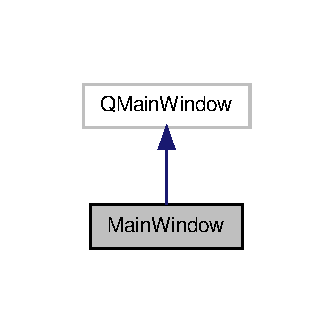
\includegraphics[width=160pt]{class_main_window__inherit__graph}
\end{center}
\end{figure}
\subsubsection*{Métodos públicos}
\begin{DoxyCompactItemize}
\item 
\hyperlink{class_main_window_a8b244be8b7b7db1b08de2a2acb9409db}{Main\-Window} (Q\-Widget $\ast$parent=0)
\begin{DoxyCompactList}\small\item\em \hyperlink{class_main_window_a8b244be8b7b7db1b08de2a2acb9409db}{Main\-Window\-::\-Main\-Window(\-Q\-Widget $\ast$parent)} Constructor. Inicializa objeto \hyperlink{class_main_window}{Main\-Window}. \end{DoxyCompactList}\item 
\hyperlink{class_main_window_ae98d00a93bc118200eeef9f9bba1dba7}{$\sim$\-Main\-Window} ()
\begin{DoxyCompactList}\small\item\em \hyperlink{class_main_window_ae98d00a93bc118200eeef9f9bba1dba7}{Main\-Window\-::$\sim$\-Main\-Window()} Destructor. \end{DoxyCompactList}\end{DoxyCompactItemize}
\subsubsection*{Slots privados}
\begin{DoxyCompactItemize}
\item 
void \hyperlink{class_main_window_a957d9751c06e3d563c12f8deac28bd0a}{ejecutar} ()
\begin{DoxyCompactList}\small\item\em \hyperlink{class_main_window_a957d9751c06e3d563c12f8deac28bd0a}{Main\-Window\-::ejecutar()} Ejecuta el algoritmo. Y actualiza los campos con los datos obtenidos con el algoritmo. \end{DoxyCompactList}\item 
void \hyperlink{class_main_window_a26d568bd0afde2853dbf4d1d376e5983}{abrir\-Archivo} ()
\begin{DoxyCompactList}\small\item\em \hyperlink{class_main_window_a26d568bd0afde2853dbf4d1d376e5983}{Main\-Window\-::abrir\-Archivo()} Este m\'{e}todo permite cargar un archivo de grafo, como primer paso para aplicar el algoritmo. \end{DoxyCompactList}\item 
void \hyperlink{class_main_window_a05df693b04b7468859a1927de1002455}{guardar\-Solucion} ()
\begin{DoxyCompactList}\small\item\em \hyperlink{class_main_window_a05df693b04b7468859a1927de1002455}{Main\-Window\-::guardar\-Solucion()} Guarda la solucion encontrada en formato {\itshape graphml}. \end{DoxyCompactList}\end{DoxyCompactItemize}
\subsubsection*{Métodos privados}
\begin{DoxyCompactItemize}
\item 
void \hyperlink{class_main_window_af241cf8ff6b2e4a17558e6487d705331}{deshabilitar\-Algoritmo} (bool habilitar)
\begin{DoxyCompactList}\small\item\em \hyperlink{class_main_window_af241cf8ff6b2e4a17558e6487d705331}{Main\-Window\-::deshabilitar\-Algoritmo} Habilita o deshabilita la opci\'{o}n de usar el algoritmo. \end{DoxyCompactList}\item 
void \hyperlink{class_main_window_a4678687dacfc0628fbb70a784eaf5ccb}{limpiar\-Datos} ()
\begin{DoxyCompactList}\small\item\em \hyperlink{class_main_window_a4678687dacfc0628fbb70a784eaf5ccb}{Main\-Window\-::limpiar\-Datos} Limpia los campos de los paneles de datos de entrada y datos de salida. \end{DoxyCompactList}\item 
void \hyperlink{class_main_window_ac851388477837047f7246785cddcd432}{destruir\-Datos} ()
\end{DoxyCompactItemize}
\subsubsection*{Atributos privados}
\begin{DoxyCompactItemize}
\item 
Ui\-::\-Main\-Window $\ast$ \hyperlink{class_main_window_a35466a70ed47252a0191168126a352a5}{ui}
\item 
\hyperlink{class_algoritmo}{Algoritmo} $\ast$ \hyperlink{class_main_window_af719c5b31f6538cfe9b91a0e3f6a3e5e}{algoritmo}
\item 
\hyperlink{class_lectora_archivo}{Lectora\-Archivo} $\ast$ \hyperlink{class_main_window_acf9c9d69b2ad41d7d536f08c5e39dd15}{lectora\-De\-Archivo}
\item 
bool \hyperlink{class_main_window_a40ea4c12346500b727bb1b56647d0b9b}{flag\-Lectora}
\item 
bool \hyperlink{class_main_window_a03312d997bf45b1429cab82fb1b1e803}{flag\-Algoritmo}
\end{DoxyCompactItemize}


\subsubsection{Descripción detallada}


Definición en la línea 20 del archivo mainwindow.\-h.



\subsubsection{Documentación del constructor y destructor}
\hypertarget{class_main_window_a8b244be8b7b7db1b08de2a2acb9409db}{\index{Main\-Window@{Main\-Window}!Main\-Window@{Main\-Window}}
\index{Main\-Window@{Main\-Window}!MainWindow@{Main\-Window}}
\paragraph[{Main\-Window}]{\setlength{\rightskip}{0pt plus 5cm}Main\-Window\-::\-Main\-Window (
\begin{DoxyParamCaption}
\item[{Q\-Widget $\ast$}]{parent = {\ttfamily 0}}
\end{DoxyParamCaption}
)\hspace{0.3cm}{\ttfamily [explicit]}}}\label{class_main_window_a8b244be8b7b7db1b08de2a2acb9409db}


\hyperlink{class_main_window_a8b244be8b7b7db1b08de2a2acb9409db}{Main\-Window\-::\-Main\-Window(\-Q\-Widget $\ast$parent)} Constructor. Inicializa objeto \hyperlink{class_main_window}{Main\-Window}. 


\begin{DoxyParams}{Parámetros}
{\em parent} & \\
\hline
\end{DoxyParams}


Definición en la línea 25 del archivo mainwindow.\-cpp.

\hypertarget{class_main_window_ae98d00a93bc118200eeef9f9bba1dba7}{\index{Main\-Window@{Main\-Window}!$\sim$\-Main\-Window@{$\sim$\-Main\-Window}}
\index{$\sim$\-Main\-Window@{$\sim$\-Main\-Window}!MainWindow@{Main\-Window}}
\paragraph[{$\sim$\-Main\-Window}]{\setlength{\rightskip}{0pt plus 5cm}Main\-Window\-::$\sim$\-Main\-Window (
\begin{DoxyParamCaption}
{}
\end{DoxyParamCaption}
)}}\label{class_main_window_ae98d00a93bc118200eeef9f9bba1dba7}


\hyperlink{class_main_window_ae98d00a93bc118200eeef9f9bba1dba7}{Main\-Window\-::$\sim$\-Main\-Window()} Destructor. 



Definición en la línea 49 del archivo mainwindow.\-cpp.



\subsubsection{Documentación de las funciones miembro}
\hypertarget{class_main_window_a26d568bd0afde2853dbf4d1d376e5983}{\index{Main\-Window@{Main\-Window}!abrir\-Archivo@{abrir\-Archivo}}
\index{abrir\-Archivo@{abrir\-Archivo}!MainWindow@{Main\-Window}}
\paragraph[{abrir\-Archivo}]{\setlength{\rightskip}{0pt plus 5cm}void Main\-Window\-::abrir\-Archivo (
\begin{DoxyParamCaption}
{}
\end{DoxyParamCaption}
)\hspace{0.3cm}{\ttfamily [private]}, {\ttfamily [slot]}}}\label{class_main_window_a26d568bd0afde2853dbf4d1d376e5983}


\hyperlink{class_main_window_a26d568bd0afde2853dbf4d1d376e5983}{Main\-Window\-::abrir\-Archivo()} Este m\'{e}todo permite cargar un archivo de grafo, como primer paso para aplicar el algoritmo. 

\begin{DoxyNote}{Nota}
Los formatos admitidos son .graphml y .txt El formato .txt corresponde al formato de edgelist de un grafo.\par
 A continuaci\'{o}n un ejemplo del formato .txt (edgelist)\-:\par
 1 2 \par
 3 6 \par
 7 8 \par
\par

\end{DoxyNote}
Para conocer m\'{a}s acerca del formato .graphml visite \href{http://graphml.graphdrawing.org/primer/graphml-primer.html}{\tt http\-://graphml.\-graphdrawing.\-org/primer/graphml-\/primer.\-html} 

Definición en la línea 157 del archivo mainwindow.\-cpp.

\hypertarget{class_main_window_af241cf8ff6b2e4a17558e6487d705331}{\index{Main\-Window@{Main\-Window}!deshabilitar\-Algoritmo@{deshabilitar\-Algoritmo}}
\index{deshabilitar\-Algoritmo@{deshabilitar\-Algoritmo}!MainWindow@{Main\-Window}}
\paragraph[{deshabilitar\-Algoritmo}]{\setlength{\rightskip}{0pt plus 5cm}void Main\-Window\-::deshabilitar\-Algoritmo (
\begin{DoxyParamCaption}
\item[{bool}]{habilitar}
\end{DoxyParamCaption}
)\hspace{0.3cm}{\ttfamily [private]}}}\label{class_main_window_af241cf8ff6b2e4a17558e6487d705331}


\hyperlink{class_main_window_af241cf8ff6b2e4a17558e6487d705331}{Main\-Window\-::deshabilitar\-Algoritmo} Habilita o deshabilita la opci\'{o}n de usar el algoritmo. 


\begin{DoxyParams}{Parámetros}
{\em habilitar} & bool \\
\hline
\end{DoxyParams}


Definición en la línea 73 del archivo mainwindow.\-cpp.

\hypertarget{class_main_window_ac851388477837047f7246785cddcd432}{\index{Main\-Window@{Main\-Window}!destruir\-Datos@{destruir\-Datos}}
\index{destruir\-Datos@{destruir\-Datos}!MainWindow@{Main\-Window}}
\paragraph[{destruir\-Datos}]{\setlength{\rightskip}{0pt plus 5cm}void Main\-Window\-::destruir\-Datos (
\begin{DoxyParamCaption}
{}
\end{DoxyParamCaption}
)\hspace{0.3cm}{\ttfamily [private]}}}\label{class_main_window_ac851388477837047f7246785cddcd432}
\hypertarget{class_main_window_a957d9751c06e3d563c12f8deac28bd0a}{\index{Main\-Window@{Main\-Window}!ejecutar@{ejecutar}}
\index{ejecutar@{ejecutar}!MainWindow@{Main\-Window}}
\paragraph[{ejecutar}]{\setlength{\rightskip}{0pt plus 5cm}void Main\-Window\-::ejecutar (
\begin{DoxyParamCaption}
{}
\end{DoxyParamCaption}
)\hspace{0.3cm}{\ttfamily [private]}, {\ttfamily [slot]}}}\label{class_main_window_a957d9751c06e3d563c12f8deac28bd0a}


\hyperlink{class_main_window_a957d9751c06e3d563c12f8deac28bd0a}{Main\-Window\-::ejecutar()} Ejecuta el algoritmo. Y actualiza los campos con los datos obtenidos con el algoritmo. 



Definición en la línea 108 del archivo mainwindow.\-cpp.

\hypertarget{class_main_window_a05df693b04b7468859a1927de1002455}{\index{Main\-Window@{Main\-Window}!guardar\-Solucion@{guardar\-Solucion}}
\index{guardar\-Solucion@{guardar\-Solucion}!MainWindow@{Main\-Window}}
\paragraph[{guardar\-Solucion}]{\setlength{\rightskip}{0pt plus 5cm}void Main\-Window\-::guardar\-Solucion (
\begin{DoxyParamCaption}
{}
\end{DoxyParamCaption}
)\hspace{0.3cm}{\ttfamily [private]}, {\ttfamily [slot]}}}\label{class_main_window_a05df693b04b7468859a1927de1002455}


\hyperlink{class_main_window_a05df693b04b7468859a1927de1002455}{Main\-Window\-::guardar\-Solucion()} Guarda la solucion encontrada en formato {\itshape graphml}. 



Definición en la línea 232 del archivo mainwindow.\-cpp.

\hypertarget{class_main_window_a4678687dacfc0628fbb70a784eaf5ccb}{\index{Main\-Window@{Main\-Window}!limpiar\-Datos@{limpiar\-Datos}}
\index{limpiar\-Datos@{limpiar\-Datos}!MainWindow@{Main\-Window}}
\paragraph[{limpiar\-Datos}]{\setlength{\rightskip}{0pt plus 5cm}void Main\-Window\-::limpiar\-Datos (
\begin{DoxyParamCaption}
{}
\end{DoxyParamCaption}
)\hspace{0.3cm}{\ttfamily [private]}}}\label{class_main_window_a4678687dacfc0628fbb70a784eaf5ccb}


\hyperlink{class_main_window_a4678687dacfc0628fbb70a784eaf5ccb}{Main\-Window\-::limpiar\-Datos} Limpia los campos de los paneles de datos de entrada y datos de salida. 



Definición en la línea 88 del archivo mainwindow.\-cpp.



\subsubsection{Documentación de los datos miembro}
\hypertarget{class_main_window_af719c5b31f6538cfe9b91a0e3f6a3e5e}{\index{Main\-Window@{Main\-Window}!algoritmo@{algoritmo}}
\index{algoritmo@{algoritmo}!MainWindow@{Main\-Window}}
\paragraph[{algoritmo}]{\setlength{\rightskip}{0pt plus 5cm}{\bf Algoritmo}$\ast$ Main\-Window\-::algoritmo\hspace{0.3cm}{\ttfamily [private]}}}\label{class_main_window_af719c5b31f6538cfe9b91a0e3f6a3e5e}


Definición en la línea 30 del archivo mainwindow.\-h.

\hypertarget{class_main_window_a03312d997bf45b1429cab82fb1b1e803}{\index{Main\-Window@{Main\-Window}!flag\-Algoritmo@{flag\-Algoritmo}}
\index{flag\-Algoritmo@{flag\-Algoritmo}!MainWindow@{Main\-Window}}
\paragraph[{flag\-Algoritmo}]{\setlength{\rightskip}{0pt plus 5cm}bool Main\-Window\-::flag\-Algoritmo\hspace{0.3cm}{\ttfamily [private]}}}\label{class_main_window_a03312d997bf45b1429cab82fb1b1e803}


Definición en la línea 35 del archivo mainwindow.\-h.

\hypertarget{class_main_window_a40ea4c12346500b727bb1b56647d0b9b}{\index{Main\-Window@{Main\-Window}!flag\-Lectora@{flag\-Lectora}}
\index{flag\-Lectora@{flag\-Lectora}!MainWindow@{Main\-Window}}
\paragraph[{flag\-Lectora}]{\setlength{\rightskip}{0pt plus 5cm}bool Main\-Window\-::flag\-Lectora\hspace{0.3cm}{\ttfamily [private]}}}\label{class_main_window_a40ea4c12346500b727bb1b56647d0b9b}


Definición en la línea 34 del archivo mainwindow.\-h.

\hypertarget{class_main_window_acf9c9d69b2ad41d7d536f08c5e39dd15}{\index{Main\-Window@{Main\-Window}!lectora\-De\-Archivo@{lectora\-De\-Archivo}}
\index{lectora\-De\-Archivo@{lectora\-De\-Archivo}!MainWindow@{Main\-Window}}
\paragraph[{lectora\-De\-Archivo}]{\setlength{\rightskip}{0pt plus 5cm}{\bf Lectora\-Archivo}$\ast$ Main\-Window\-::lectora\-De\-Archivo\hspace{0.3cm}{\ttfamily [private]}}}\label{class_main_window_acf9c9d69b2ad41d7d536f08c5e39dd15}


Definición en la línea 31 del archivo mainwindow.\-h.

\hypertarget{class_main_window_a35466a70ed47252a0191168126a352a5}{\index{Main\-Window@{Main\-Window}!ui@{ui}}
\index{ui@{ui}!MainWindow@{Main\-Window}}
\paragraph[{ui}]{\setlength{\rightskip}{0pt plus 5cm}Ui\-::\-Main\-Window$\ast$ Main\-Window\-::ui\hspace{0.3cm}{\ttfamily [private]}}}\label{class_main_window_a35466a70ed47252a0191168126a352a5}


Definición en la línea 29 del archivo mainwindow.\-h.



La documentación para esta clase fue generada a partir de los siguientes ficheros\-:\begin{DoxyCompactItemize}
\item 
clustering/\hyperlink{mainwindow_8h}{mainwindow.\-h}\item 
clustering/\hyperlink{mainwindow_8cpp}{mainwindow.\-cpp}\end{DoxyCompactItemize}

\section{Documentación de archivos}
\hypertarget{algoritmo_8cpp}{\subsection{Referencia del Archivo clustering/algoritmo.cpp}
\label{algoritmo_8cpp}\index{clustering/algoritmo.\-cpp@{clustering/algoritmo.\-cpp}}
}


Implementaci\'{o}n de los mtodos de la clase \hyperlink{class_algoritmo}{Algoritmo}.  


{\ttfamily \#include \char`\"{}algoritmo.\-h\char`\"{}}\\*
{\ttfamily \#include $<$Q\-String$>$}\\*
{\ttfamily \#include $<$math.\-h$>$}\\*
{\ttfamily \#include $<$iostream$>$}\\*
Dependencia gráfica adjunta para algoritmo.\-cpp\-:\nopagebreak
\begin{figure}[H]
\begin{center}
\leavevmode
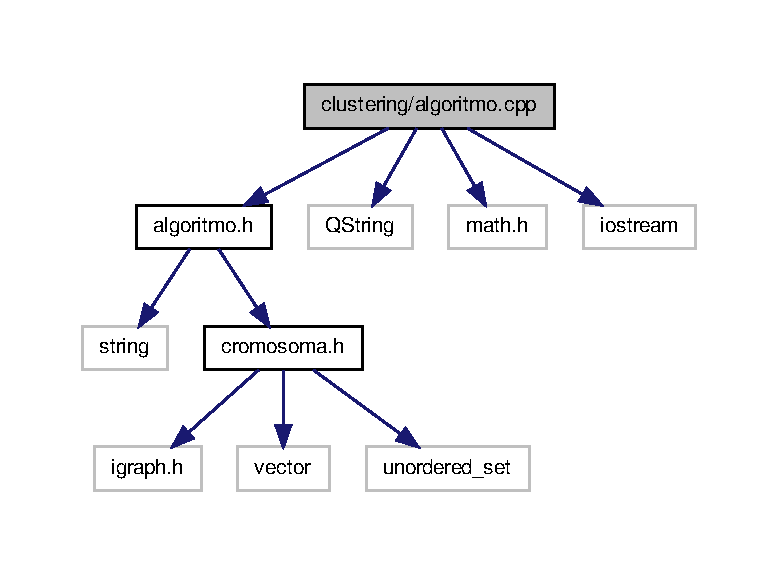
\includegraphics[width=350pt]{algoritmo_8cpp__incl}
\end{center}
\end{figure}


\subsubsection{Descripción detallada}
Implementaci\'{o}n de los mtodos de la clase \hyperlink{class_algoritmo}{Algoritmo}. \begin{DoxyAuthor}{Autor}
Mar\'{\i}a Andrea Cruz Bland\'{o}n 
\end{DoxyAuthor}
\begin{DoxyDate}{Fecha}
09/2013, 11/2013 
\end{DoxyDate}


Definición en el archivo \hyperlink{algoritmo_8cpp_source}{algoritmo.\-cpp}.


\hypertarget{algoritmo_8h}{\subsection{Referencia del Archivo clustering/algoritmo.h}
\label{algoritmo_8h}\index{clustering/algoritmo.\-h@{clustering/algoritmo.\-h}}
}


Definici\'{o}n de la clase \hyperlink{class_algoritmo}{Algoritmo}.  


{\ttfamily \#include $<$string$>$}\\*
{\ttfamily \#include \char`\"{}cromosoma.\-h\char`\"{}}\\*
Dependencia gráfica adjunta para algoritmo.\-h\-:\nopagebreak
\begin{figure}[H]
\begin{center}
\leavevmode
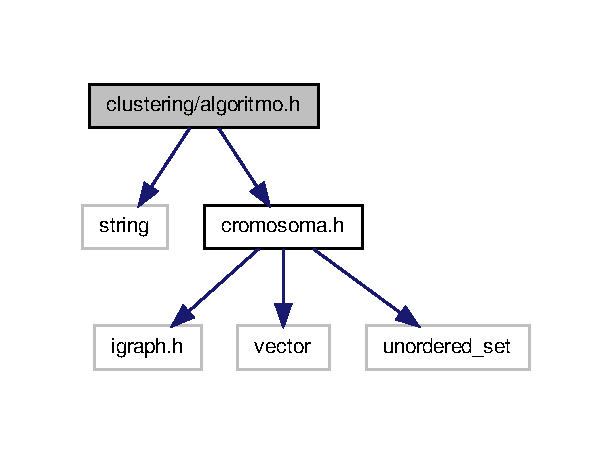
\includegraphics[width=294pt]{algoritmo_8h__incl}
\end{center}
\end{figure}
Gráfico de los archivos que directa o indirectamente incluyen a este archivo\-:\nopagebreak
\begin{figure}[H]
\begin{center}
\leavevmode
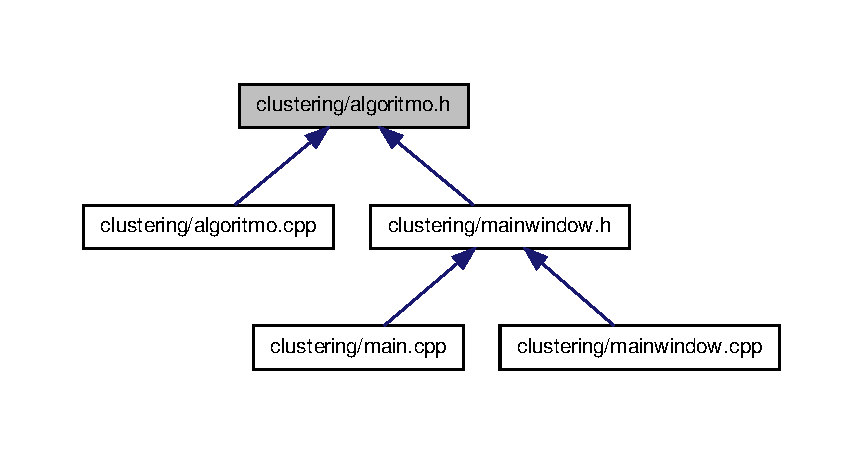
\includegraphics[width=350pt]{algoritmo_8h__dep__incl}
\end{center}
\end{figure}
\subsubsection*{Clases}
\begin{DoxyCompactItemize}
\item 
class \hyperlink{class_algoritmo}{Algoritmo}
\end{DoxyCompactItemize}


\subsubsection{Descripción detallada}
Definici\'{o}n de la clase \hyperlink{class_algoritmo}{Algoritmo}. \begin{DoxyAuthor}{Autor}
Mar\'{\i}a Andrea Cruz Bland\'{o}n 
\end{DoxyAuthor}
\begin{DoxyDate}{Fecha}
09/2013, 11/2013 
\end{DoxyDate}


Definición en el archivo \hyperlink{algoritmo_8h_source}{algoritmo.\-h}.


\hypertarget{cromosoma_8cpp}{\subsection{Referencia del Archivo clustering/cromosoma.cpp}
\label{cromosoma_8cpp}\index{clustering/cromosoma.\-cpp@{clustering/cromosoma.\-cpp}}
}


Implementaci\'{o}n de los mtodos de la clase \hyperlink{class_cromosoma}{Cromosoma}.  


{\ttfamily \#include \char`\"{}cromosoma.\-h\char`\"{}}\\*
{\ttfamily \#include $<$iostream$>$}\\*
Dependencia gráfica adjunta para cromosoma.\-cpp\-:\nopagebreak
\begin{figure}[H]
\begin{center}
\leavevmode
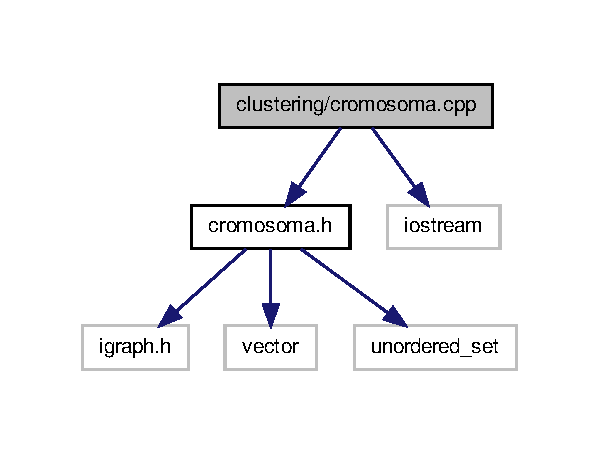
\includegraphics[width=288pt]{cromosoma_8cpp__incl}
\end{center}
\end{figure}


\subsubsection{Descripción detallada}
Implementaci\'{o}n de los mtodos de la clase \hyperlink{class_cromosoma}{Cromosoma}. \begin{DoxyAuthor}{Autor}
Mar\'{\i}a Andrea Cruz Bland\'{o}n 
\end{DoxyAuthor}
\begin{DoxyDate}{Fecha}
09/2013, 11/2013 
\end{DoxyDate}


Definición en el archivo \hyperlink{cromosoma_8cpp_source}{cromosoma.\-cpp}.


\hypertarget{cromosoma_8h}{\subsection{Referencia del Archivo clustering/cromosoma.h}
\label{cromosoma_8h}\index{clustering/cromosoma.\-h@{clustering/cromosoma.\-h}}
}


Definici\'{o}n de la clase \hyperlink{class_cromosoma}{Cromosoma}.  


{\ttfamily \#include $<$igraph.\-h$>$}\\*
{\ttfamily \#include $<$vector$>$}\\*
{\ttfamily \#include $<$unordered\-\_\-set$>$}\\*
Dependencia gráfica adjunta para cromosoma.\-h\-:\nopagebreak
\begin{figure}[H]
\begin{center}
\leavevmode
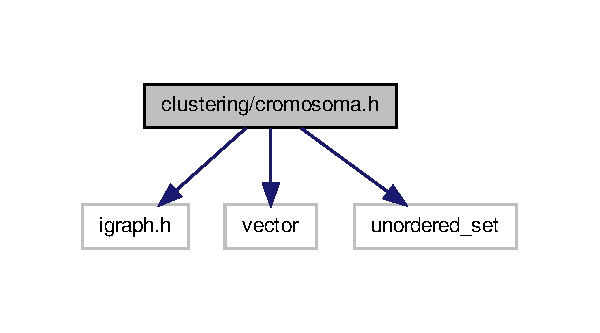
\includegraphics[width=288pt]{cromosoma_8h__incl}
\end{center}
\end{figure}
Gráfico de los archivos que directa o indirectamente incluyen a este archivo\-:\nopagebreak
\begin{figure}[H]
\begin{center}
\leavevmode
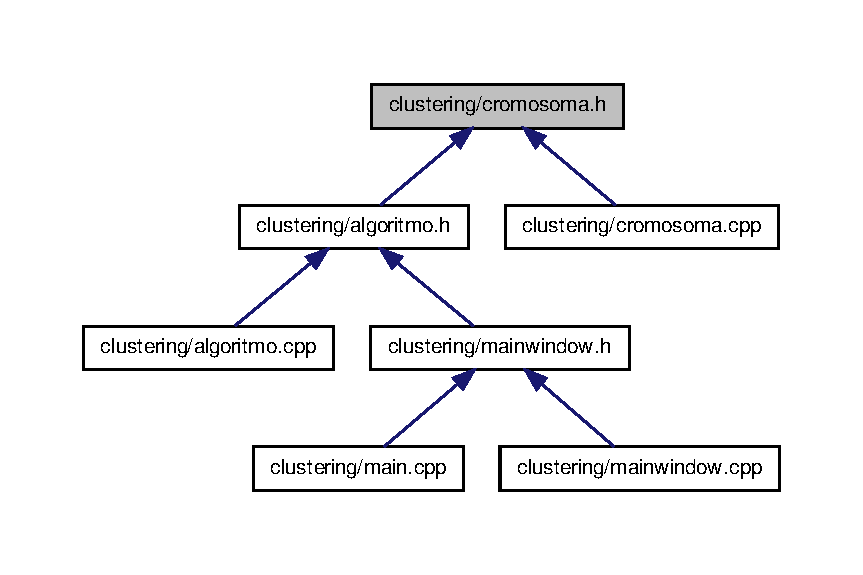
\includegraphics[width=350pt]{cromosoma_8h__dep__incl}
\end{center}
\end{figure}
\subsubsection*{Clases}
\begin{DoxyCompactItemize}
\item 
class \hyperlink{class_cromosoma}{Cromosoma}
\end{DoxyCompactItemize}


\subsubsection{Descripción detallada}
Definici\'{o}n de la clase \hyperlink{class_cromosoma}{Cromosoma}. \begin{DoxyAuthor}{Autor}
Mar\'{\i}a Andrea Cruz Bland\'{o}n 
\end{DoxyAuthor}
\begin{DoxyDate}{Fecha}
09/2013, 11/2013 
\end{DoxyDate}


Definición en el archivo \hyperlink{cromosoma_8h_source}{cromosoma.\-h}.


\hypertarget{lectoraarchivo_8cpp}{\subsection{Referencia del Archivo clustering/lectoraarchivo.cpp}
\label{lectoraarchivo_8cpp}\index{clustering/lectoraarchivo.\-cpp@{clustering/lectoraarchivo.\-cpp}}
}


Implementaci\'{o}n de los mtodos de la clase \hyperlink{class_lectora_archivo}{Lectora\-Archivo}.  


{\ttfamily \#include \char`\"{}lectoraarchivo.\-h\char`\"{}}\\*
{\ttfamily \#include $<$iostream$>$}\\*
{\ttfamily \#include $<$Q\-String$>$}\\*
{\ttfamily \#include $<$assert.\-h$>$}\\*
Dependencia gráfica adjunta para lectoraarchivo.\-cpp\-:\nopagebreak
\begin{figure}[H]
\begin{center}
\leavevmode
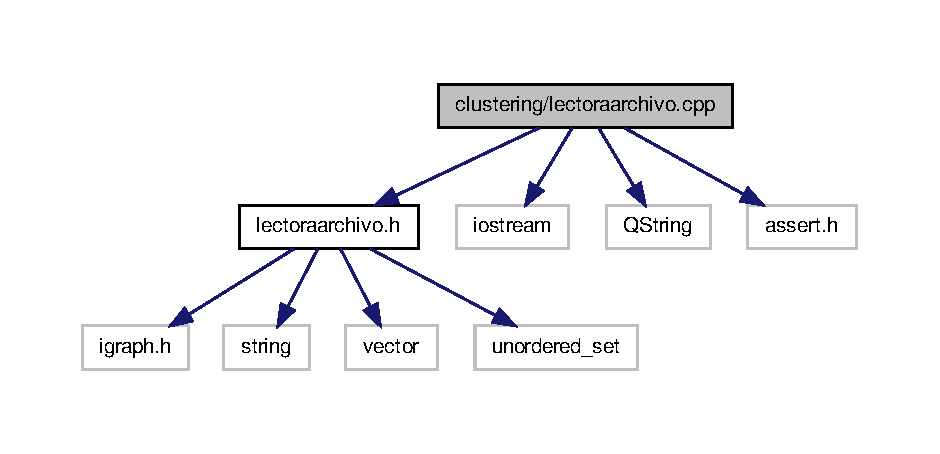
\includegraphics[width=350pt]{lectoraarchivo_8cpp__incl}
\end{center}
\end{figure}


\subsubsection{Descripción detallada}
Implementaci\'{o}n de los mtodos de la clase \hyperlink{class_lectora_archivo}{Lectora\-Archivo}. \begin{DoxyAuthor}{Autor}
Mar\'{\i}a Andrea Cruz Bland\'{o}n 
\end{DoxyAuthor}
\begin{DoxyDate}{Fecha}
09/2013, 11/2013 
\end{DoxyDate}


Definición en el archivo \hyperlink{lectoraarchivo_8cpp_source}{lectoraarchivo.\-cpp}.


\hypertarget{lectoraarchivo_8h}{\subsection{Referencia del Archivo clustering/lectoraarchivo.h}
\label{lectoraarchivo_8h}\index{clustering/lectoraarchivo.\-h@{clustering/lectoraarchivo.\-h}}
}


Definici\'{o}n de la clase \hyperlink{class_lectora_archivo}{Lectora\-Archivo}.  


{\ttfamily \#include $<$igraph.\-h$>$}\\*
{\ttfamily \#include $<$string$>$}\\*
{\ttfamily \#include $<$vector$>$}\\*
{\ttfamily \#include $<$unordered\-\_\-set$>$}\\*
Dependencia gráfica adjunta para lectoraarchivo.\-h\-:\nopagebreak
\begin{figure}[H]
\begin{center}
\leavevmode
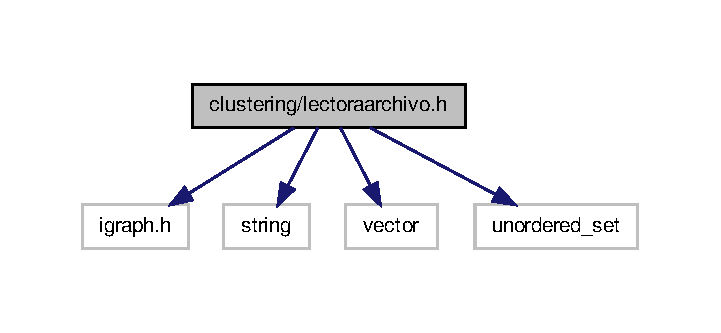
\includegraphics[width=346pt]{lectoraarchivo_8h__incl}
\end{center}
\end{figure}
Gráfico de los archivos que directa o indirectamente incluyen a este archivo\-:\nopagebreak
\begin{figure}[H]
\begin{center}
\leavevmode
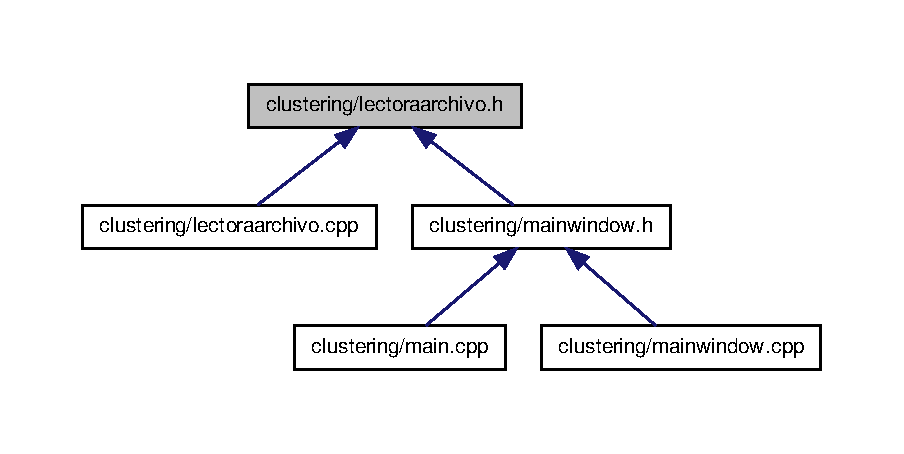
\includegraphics[width=350pt]{lectoraarchivo_8h__dep__incl}
\end{center}
\end{figure}
\subsubsection*{Clases}
\begin{DoxyCompactItemize}
\item 
class \hyperlink{class_lectora_archivo}{Lectora\-Archivo}
\end{DoxyCompactItemize}


\subsubsection{Descripción detallada}
Definici\'{o}n de la clase \hyperlink{class_lectora_archivo}{Lectora\-Archivo}. \begin{DoxyAuthor}{Autor}
Mar\'{\i}a Andrea Cruz Bland\'{o}n 
\end{DoxyAuthor}
\begin{DoxyDate}{Fecha}
09/2013, 11/2013 
\end{DoxyDate}


Definición en el archivo \hyperlink{lectoraarchivo_8h_source}{lectoraarchivo.\-h}.


\hypertarget{main_8cpp}{\subsection{Referencia del Archivo clustering/main.cpp}
\label{main_8cpp}\index{clustering/main.\-cpp@{clustering/main.\-cpp}}
}


Archivo principal del proyecto.  


{\ttfamily \#include \char`\"{}mainwindow.\-h\char`\"{}}\\*
{\ttfamily \#include $<$Q\-Application$>$}\\*
{\ttfamily \#include $<$time.\-h$>$}\\*
Dependencia gráfica adjunta para main.\-cpp\-:\nopagebreak
\begin{figure}[H]
\begin{center}
\leavevmode
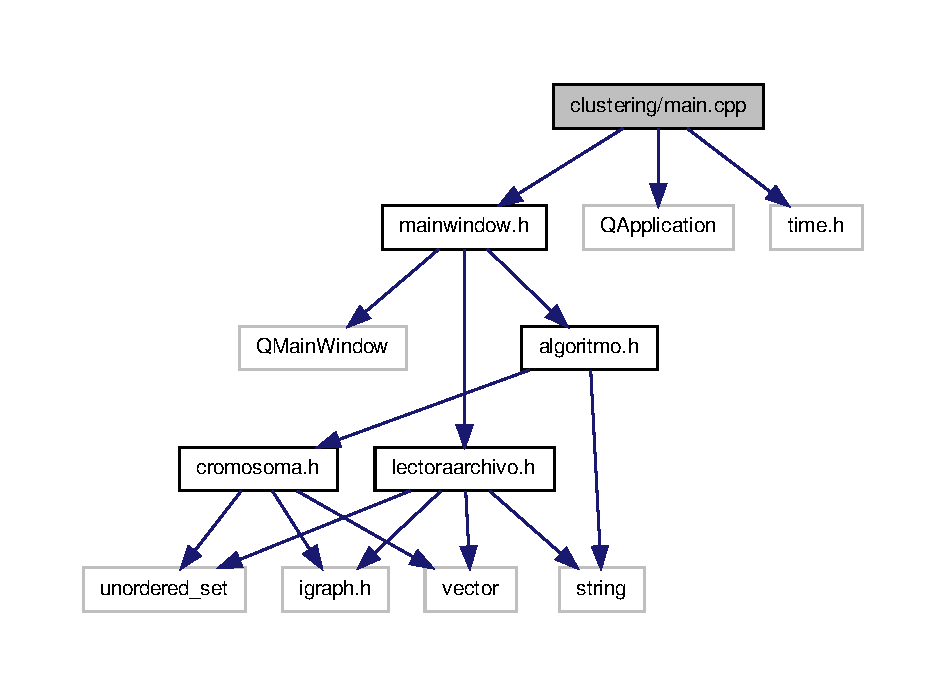
\includegraphics[width=350pt]{main_8cpp__incl}
\end{center}
\end{figure}
\subsubsection*{Funciones}
\begin{DoxyCompactItemize}
\item 
int \hyperlink{main_8cpp_a0ddf1224851353fc92bfbff6f499fa97}{main} (int argc, char $\ast$argv\mbox{[}$\,$\mbox{]})
\begin{DoxyCompactList}\small\item\em main Se inicializa la aplicaci\'{o}n. \end{DoxyCompactList}\end{DoxyCompactItemize}


\subsubsection{Descripción detallada}
Archivo principal del proyecto. \begin{DoxyAuthor}{Autor}
Mar\'{\i}a Andrea Cruz Bland\'{o}n 
\end{DoxyAuthor}
\begin{DoxyDate}{Fecha}
09/2013, 11/2013 
\end{DoxyDate}


Definición en el archivo \hyperlink{main_8cpp_source}{main.\-cpp}.



\subsubsection{Documentación de las funciones}
\hypertarget{main_8cpp_a0ddf1224851353fc92bfbff6f499fa97}{\index{main.\-cpp@{main.\-cpp}!main@{main}}
\index{main@{main}!main.cpp@{main.\-cpp}}
\paragraph[{main}]{\setlength{\rightskip}{0pt plus 5cm}int main (
\begin{DoxyParamCaption}
\item[{int}]{argc, }
\item[{char $\ast$}]{argv\mbox{[}$\,$\mbox{]}}
\end{DoxyParamCaption}
)}}\label{main_8cpp_a0ddf1224851353fc92bfbff6f499fa97}


main Se inicializa la aplicaci\'{o}n. 

\begin{DoxyNote}{Nota}
En algoritmo geneticos es recomendables s\'{o}lo ejecutar la inicializacion del Rand una vez en toda la ejecuci\'{o}n del algoritmo.
\end{DoxyNote}


Definición en la línea 27 del archivo main.\-cpp.


\hypertarget{mainwindow_8cpp}{\subsection{Referencia del Archivo clustering/mainwindow.cpp}
\label{mainwindow_8cpp}\index{clustering/mainwindow.\-cpp@{clustering/mainwindow.\-cpp}}
}


Implementaci\'{o}n de los mtodos de la clase \hyperlink{class_main_window}{Main\-Window}.  


{\ttfamily \#include \char`\"{}mainwindow.\-h\char`\"{}}\\*
{\ttfamily \#include \char`\"{}ui\-\_\-mainwindow.\-h\char`\"{}}\\*
{\ttfamily \#include $<$Q\-Message\-Box$>$}\\*
{\ttfamily \#include $<$Q\-File\-Dialog$>$}\\*
{\ttfamily \#include $<$iostream$>$}\\*
Dependencia gráfica adjunta para mainwindow.\-cpp\-:\nopagebreak
\begin{figure}[H]
\begin{center}
\leavevmode
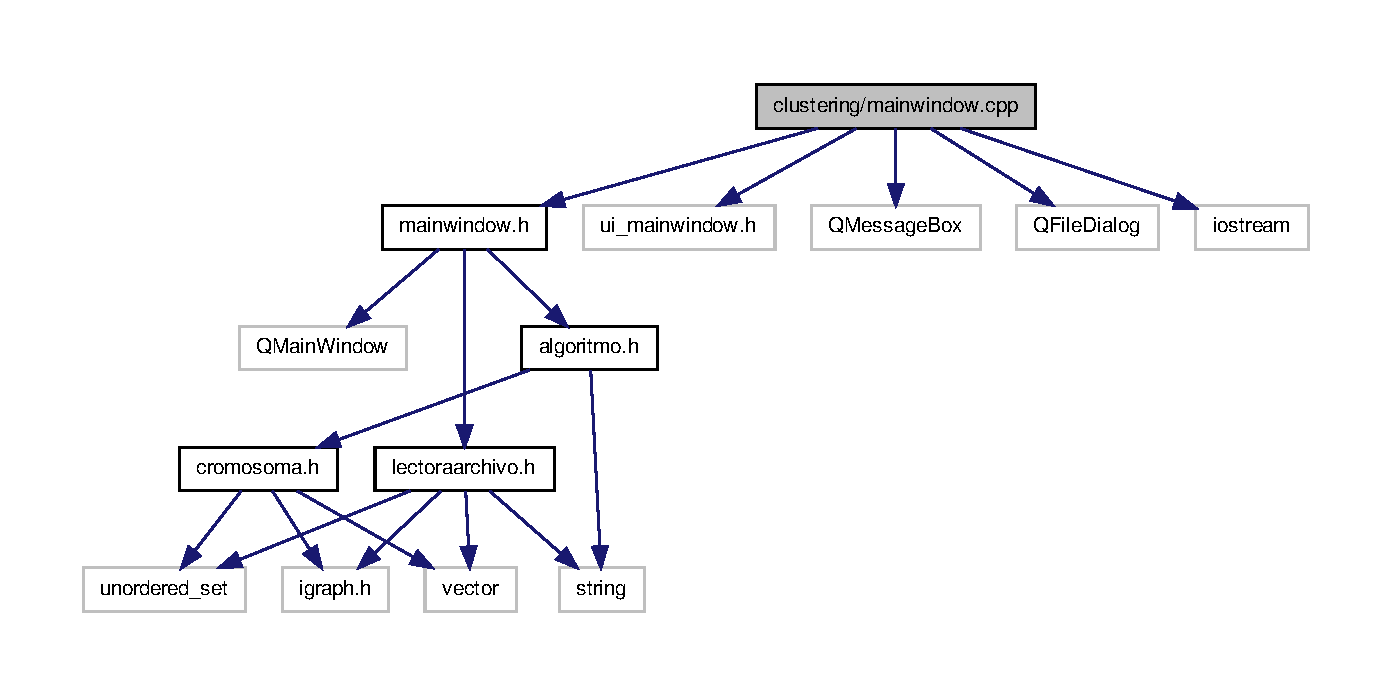
\includegraphics[width=350pt]{mainwindow_8cpp__incl}
\end{center}
\end{figure}


\subsubsection{Descripción detallada}
Implementaci\'{o}n de los mtodos de la clase \hyperlink{class_main_window}{Main\-Window}. \begin{DoxyAuthor}{Autor}
Mar\'{\i}a Andrea Cruz Bland\'{o}n 
\end{DoxyAuthor}
\begin{DoxyDate}{Fecha}
09/2013, 11/2013 
\end{DoxyDate}


Definición en el archivo \hyperlink{mainwindow_8cpp_source}{mainwindow.\-cpp}.


\hypertarget{mainwindow_8h}{\subsection{Referencia del Archivo clustering/mainwindow.h}
\label{mainwindow_8h}\index{clustering/mainwindow.\-h@{clustering/mainwindow.\-h}}
}


Definici\'{o}n de la clase \hyperlink{class_main_window}{Main\-Window}.  


{\ttfamily \#include $<$Q\-Main\-Window$>$}\\*
{\ttfamily \#include \char`\"{}algoritmo.\-h\char`\"{}}\\*
{\ttfamily \#include \char`\"{}lectoraarchivo.\-h\char`\"{}}\\*
Dependencia gráfica adjunta para mainwindow.\-h\-:\nopagebreak
\begin{figure}[H]
\begin{center}
\leavevmode
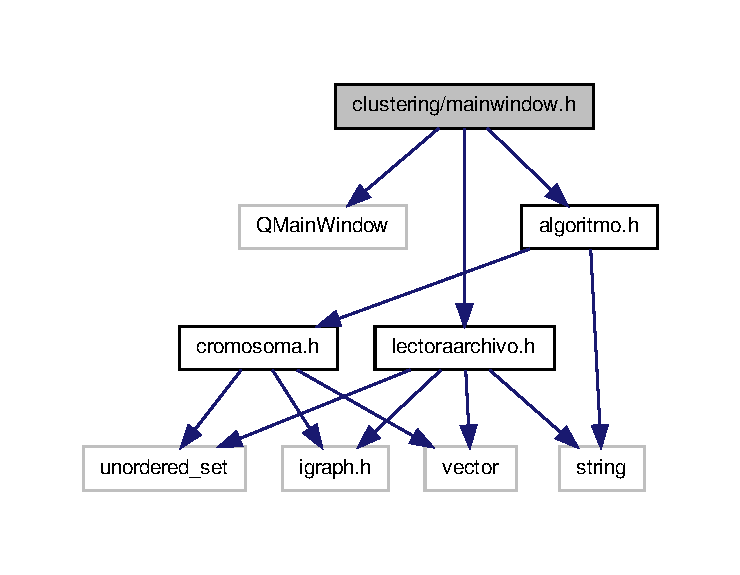
\includegraphics[width=350pt]{mainwindow_8h__incl}
\end{center}
\end{figure}
Gráfico de los archivos que directa o indirectamente incluyen a este archivo\-:\nopagebreak
\begin{figure}[H]
\begin{center}
\leavevmode
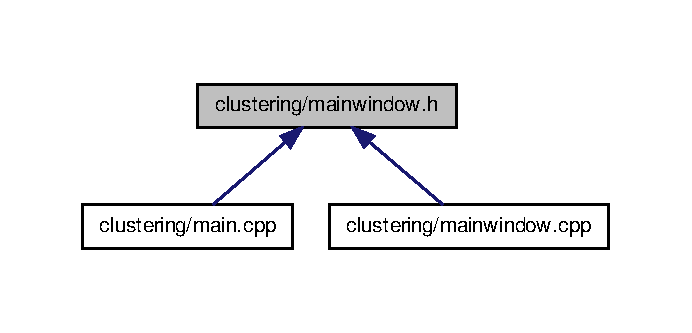
\includegraphics[width=332pt]{mainwindow_8h__dep__incl}
\end{center}
\end{figure}
\subsubsection*{Clases}
\begin{DoxyCompactItemize}
\item 
class \hyperlink{class_main_window}{Main\-Window}
\end{DoxyCompactItemize}
\subsubsection*{Namespaces}
\begin{DoxyCompactItemize}
\item 
\hyperlink{namespace_ui}{Ui}
\end{DoxyCompactItemize}
\subsubsection*{Constant Groups}
\begin{DoxyCompactItemize}
\item 
\hyperlink{namespace_ui}{Ui}
\end{DoxyCompactItemize}


\subsubsection{Descripción detallada}
Definici\'{o}n de la clase \hyperlink{class_main_window}{Main\-Window}. \begin{DoxyAuthor}{Autor}
Mar\'{\i}a Andrea Cruz Bland\'{o}n 
\end{DoxyAuthor}
\begin{DoxyDate}{Fecha}
09/2013, 11/2013 
\end{DoxyDate}


Definición en el archivo \hyperlink{mainwindow_8h_source}{mainwindow.\-h}.


%--- End generated contents ---

% Index
\newpage
\phantomsection
\addcontentsline{toc}{part}{Índice}
\printindex

\end{document}
